%
% This is file `elsarticle-template-num.tex',
% generated with the docstrip utility.
%
% The original source files were:
%
% elsarticle.dtx  (with options: `numtemplate')
% 
% Copyright 2007, 2008 Elsevier Ltd.
% 
% This file is part of the 'Elsarticle Bundle'.
% -------------------------------------------
% 
% It may be distributed under the conditions of the LaTeX Project Public
% License, either version 1.2 of this license or (at your option) any
% later version.  The latest version of this license is in
%    http://www.latex-project.org/lppl.txt
% and version 1.2 or later is part of all distributions of LaTeX
% version 1999/12/01 or later.
% 
% The list of all files belonging to the 'Elsarticle Bundle' is
% given in the file `manifest.txt'.

\documentclass[preprint,10pt]{elsarticle}

%%%%%%%%%%%%%%%%%%%%%%%%%%%%%%%%%%%%%%%%%%%%%%%%%%%%%%%%%%%%%%%%%%%%
%
%=================================================================================================
% new commands
% +++++++++++++++++++++++++++++++++++++++++++++++++++++++++++++++++++++++++++++++++++++++++++++++++
\newcommand{\nc}{\newcommand}

\renewcommand{\div}{\mbold{\nabla}\! \cdot \!}
\newcommand{\grad}{\mbold{\nabla}}
\newcommand{\divv}[1]{\boldsymbol{\nabla}^{#1}\! \cdot \!}
\newcommand{\gradd}[1]{\mbold{\nabla}^{#1}}
\newcommand{\mbold}[1]{\boldsymbol#1}
% latex shortcuts
\newcommand{\bea}{\begin{eqnarray}}
\newcommand{\eea}{\end{eqnarray}}
\newcommand{\be}{\begin{equation}}
\newcommand{\ee}{\end{equation}}
\newcommand{\bal}{\begin{align}}
\newcommand{\eali}{\end{align}}
\newcommand{\bi}{\begin{itemize}}
\newcommand{\ei}{\end{itemize}}
\newcommand{\ben}{\begin{enumerate}}
\newcommand{\een}{\end{enumerate}}
\usepackage{amsthm}
\newtheorem*{remark}{Remark}
% DGFEM commands
\newcommand{\jmp}[1]{[\![#1]\!]}                     % jump
\newcommand{\mvl}[1]{\{\!\!\{#1\}\!\!\}}             % mean value
\newcommand{\keff}{\ensuremath{k_{\textit{eff}}}\xspace}
% shortcut for domain notation
\newcommand{\D}{\mathcal{D}}
% vector shortcuts
\newcommand{\vo}{\mbold{\Omega}}
\newcommand{\vr}{\mbold{r}}
\newcommand{\vn}{\mbold{n}}
\newcommand{\vnk}{\mbold{\mathbf{n}}}
\newcommand{\vj}{\mbold{J}}
\newcommand{\eig}[1]{\| #1 \|_2}
%
\newcommand{\EI}{\mathcal{E}_h^i}
\newcommand{\ED}{\mathcal{E}_h^{\partial \D^d}}
\newcommand{\EN}{\mathcal{E}_h^{\partial \D^n}}
\newcommand{\ER}{\mathcal{E}_h^{\partial \D^r}}
\newcommand{\reg}{\textit{reg}}
%
\newcommand{\norm}{\textrm{norm}}
\renewcommand{\Re}{\textrm{Re}}
\newcommand{\Pe}{\textrm{P\'e}}
\renewcommand{\Pr}{\textrm{Pr}}
%
\newcommand{\resi}{R}
%\newcommand{\resinew}{\tilde{D}_e}
\newcommand{\resinew}{\widetilde{\resi}}
\newcommand{\resisource}{\widetilde{\resi}^{source}}
\newcommand{\matder}[1]{\frac{\textrm{D} #1}{\textrm{D} t}}
%
\newcommand{\Gammakj}{\Gamma_{k \to j}}

% extra space
\newcommand{\qq}{\quad\quad}
% common reference commands
\newcommand{\eqt}[1]{Eq.~(\ref{#1})}                     % equation
\newcommand{\eqts}[1]{Eqs.~(\ref{#1})}                     % equations
\newcommand{\fig}[1]{Fig.~\ref{#1}}                      % figure
\newcommand{\tbl}[1]{Table~\ref{#1}}                     % table
\newcommand{\sct}[1]{Section~\ref{#1}}                   % section
\newcommand{\app}[1]{Appendix~\ref{#1}}                   % appendix
\newcommand{\lem}[1]{Lemma~\ref{#1}}                   % lemma
\newcommand{\theo}[1]{Theorem~\ref{#1}}                   % theorem
%
\newcommand{\ie}{i.e.,\@\xspace}
\newcommand{\eg}{e.g.,\@\xspace}
\newcommand{\psc}[1]{{\sc {#1}}}
\newcommand{\rs}{\psc{R7}\xspace}
%
\newcommand\br{\mathbf{r}}
%\newcommand{\tf}{\varphi}
\newcommand{\tf}{b}
%
%\renewcommand{\dim}{\ensuremath{\texttt{dim}}\xspace}
%
\newcommand{\tcr}[1]{\textcolor{red}{#1}}
\newcommand{\tcb}[1]{\textcolor{blue}{#1}}
  \newcommand{\tcg}[1]{\textcolor{green}{#1}}
\newcommand{\mt}[1]{\marginpar{ {\tiny #1}}}

\newtheorem{theorem}{Theorem}[section]
\newtheorem{lemma}[theorem]{Lemma}
%  various packages that you may wish to activate for usage 
\usepackage{graphicx}
\usepackage{tabls}
\usepackage{afterpage}
\usepackage{amsmath}
\usepackage{amsfonts}
\usepackage{amssymb}
\usepackage{amstext}
\usepackage{amsbsy}
\usepackage{epsfig}
%\usepackage{epsfig}
%\usepackage{cites}
\usepackage{epsf}

\usepackage{array}
\usepackage{color}
\usepackage[section]{placeins} % force � mettre l'image o� on veut
\usepackage{float} %utiliser H pour forcer � mettre l'image o� on veut
\usepackage{lscape} %utilisation du mode paysage

%
% de dk:
%
%%\usepackage[dvips]{epsfig}
%%\usepackage[dvips]{graphicx}
%%\usepackage{comment}
%%\usepackage{floatfig}
%%\usepackage{lscape}
%%\usepackage{landscape}
%%\usepackage{graphics}
%%\usepackage{hhline}[]
%%\usepackage{latexsym}
%%\usepackage{tabularx}[]
%%\usepackage{layout}
%
% de btp:
%
%%\usepackage{fancyheadings}
%%\usepackage{minitoc}
%%\usepackage{rotating}
%% \usepackage{rotate}
%%\usepackage{subfigure}
%%\usepackage{mathaccent}
%%\usepackage{isolatin1}
%
%%\usepackage{xspace}
%%\usepackage{longtable}
%%\usepackage{caption2}
%%\usepackage{ifthen}
%
%%%%%%%%%%%%%%%%%%%%%%%%%%%%%%%%%%%%%%%%%%%%%%%%%%%%%%%%%%%%%%%%%%%%
\bibliographystyle{elsarticle-num}
%%%%%%%%%%%%%%%%%%%%%%%%%%%%%%%%%%%%%%%%%%%%%%%%%%%%%%%%%%%%%%%%%%%%%
%
%   BEGIN DOCUMENT
%
%%%%%%%%%%%%%%%%%%%%%%%%%%%%%%%%%%%%%%%%%%%%%%%%%%%%%%%%%%%%%%%%%%%%%
\begin{document}

%%%%%%%%%%%%%%%%%%%%%%%%%%%%%%%%%%%%%%%%%%%%%%%%%%%%%%%%%%%%%%%%%%%%
\begin{frontmatter}

%% Title, authors and addresses

%% use the tnoteref command within \title for footnotes;
%% use the tnotetext command for theassociated footnote;
%% use the fnref command within \author or \address for footnotes;
%% use the fntext command for theassociated footnote;
%% use the corref command within \author for corresponding author footnotes;
%% use the cortext command for theassociated footnote;
%% use the ead command for the email address,
%% and the form \ead[url] for the home page:
%\title{Title\tnoteref{label1}}
%% \tnotetext[label1]{}
%% \author{Name\corref{cor1}\fnref{label2}}
%% \ead{email address}
%% \ead[url]{home page}
%% \fntext[label2]{}
%% \cortext[cor1]{}
%% \address{Address\fnref{label3}}
%% \fntext[label3]{}
%-------------------------
%-------------------------
\title{$1$-D numerical results of the Seven-Equation two-phase flow Model with the entropy viscosity method.}
%-------------------------
%-------------------------
\author{Marc O. Delchini\fnref{label1}}
\ead{delchmo@tamu.edu}

\author{Jean C. Ragusa\corref{cor1}\fnref{label1}}
\ead{jean.ragusa@tamu.edu}

\author{Ray A. Berry\fnref{label2}}
\ead{ray.berry@inl.gov}

\address[label1]{Department of Nuclear Engineering, Texas A\&M University, College Station, TX 77843, USA \fnref{label1}}

\address[label2]{Idaho National Laboratory, Idaho Falls, ID 83415, USA \fnref{label2}}

\cortext[cor1]{Corresponding author}
%-------------------------
%-------------------------
%-------------------------
\begin{abstract}
blabla
\end{abstract}
%-------------------------
%-------------------------
\begin{keyword}
  two-phase flow model \sep 
	% with variable area \sep 
	entropy viscosity method \sep 
	artificial viscosity \sep 
	low-Mach regime \sep 
	shock-capturing .
\end{keyword}
%-------------------------
\end{frontmatter}
\linenumbers

\tcr{make sure you hit return and go to the next line often enough. Word wrapping is nice and you think we do not need to hit 
return but when I look for differences on github, it is a pain to have very long lines. thanks.}

%%%%%%%%%%%%%%%%%%%%%%%%%%%%%%%%%%%%%%%%%%%%%%%%%%%%%%%%%%%%%%%%%%%%%%%%%%%%%
\section{Introduction}\label{sec:intro}
%%%%%%%%%%%%%%%%%%%%%%%%%%%%%%%%%%%%%%%%%%%%%%%%%%%%%%%%%%%%%%%%%%%%%%%%%%%%%

\begin{itemize}
\item a few lines about the need for accurately resolving two-phase flows \tcr{borrow some for the previous 2 papers, but also we need a strong emphasis on 
2-phase flows}
\item background on the different two-phase flow models: 5-, 6- and 7-equation two-phase flow models \tcr{this is really important, we need to show we have 
read some of the 
important papers, e.g., Saurel's, by providing a 1-3 sentence resume of each of the important papers we quote.}
\item then, focus on the different types of 7-equation two-phase flow models: they mostly differ because of the closure relaxations used
\item discuss the different numerical solvers developed for the 7-equation two-phase flow model: HLL, HLLC, and approximated Riemann solvers accounting 
for the source terms
\item emphasize the fact that the above numerical solvers only works for discontinuous schemes
\item then, introduce the entropy viscosity method and details the organization of the paper 
\item explain that the entropy viscosity method requires two steps: first a viscous regularization (done in REF) and then definition of the viscosity coefficients 
(done in section ...). (IMPORTANT)
\end{itemize}

%%%%%%%%%%%%%%%%%%%%%%%%%%%%%%%%%%%%%%%%%%%%%%%%%%%%%%%%%%%%%%%%%%%%%%%%%%%%%
%%%%%%%%%%%%%%%%%%%%%%%%%%%%%%%%%%%%%%%%%%%%%%%%%%%%%%%%%%%%%%%%%%%%%%%%%%%%%
\section{The regularized Seven-Equation two-phase flow Model with an all-Mach flow viscous regularization}\label{sec:7-equ-model}
%%%%%%%%%%%%%%%%%%%%%%%%%%%%%%%%%%%%%%%%%%%%%%%%%%%%%%%%%%%%%%%%%%%%%%%%%%%%%
%%%%%%%%%%%%%%%%%%%%%%%%%%%%%%%%%%%%%%%%%%%%%%%%%%%%%%%%%%%%%%%%%%%%%%%%%%%%%

\tcr{I/you will add a short intro to re-emphasize that visc. reg. is present and what that means...\\} \tcb{done}

In this section, the inviscid Seven-Equation two-phase flow Model employed in this paper is presented along with the closure relations used to compute the 
relaxation terms and 
interfacial variables (REF). Then, expression of the artificial dissipative fluxes used in the viscous regularization are recalled. The viscous regularization was 
derived in (REF) by 
using an entropy condition called ``the minimum entropy principle" which ensures both uniqueness of the numerical solution and convergence to the physical 
solution. This section 
ends with the derivation of the phasic viscosity coefficients based on the study of the non-dimensional form of the regularized Seven-Equation two-phase flow 
Model that was 
performed in (REF). In the remaining of the paper, the spatial and temporal dependencies in each variable are omitted for conciseness. All variables are 
assumed to be spatial 
and temporal dependent but when stated otherwise. 
%
%----------------------------------------------------------------------------------------------------------------------------------
\subsection{The inviscid Seven-Equation two-phase flow Model}
%----------------------------------------------------------------------------------------------------------------------------------
%
The Seven-Equation two-phase flow Model employed in this paper is obtained by assuming that each phase satisfies the single-phase Euler 
equations (with phase-exchange terms) and by integrating the latter over a control volume after multiplication by a phasic characteristic 
function. The detailed derivation of the governing equations for a phase $k$ in interaction with a phase $j$ can be found in \cite{SEM}. 
In the SEM, each phase obeys a mass, a momentum and an energy balance equation, supplemented by an equation for the volume fraction as shown in 
\eqt{eq:7-eqn}.
%
\begin{subequations}\label{eq:7-eqn}
\begin{align}
  % liquid volume fraction
  \label{eqn:multi-d-7-eqn-vf}
  \frac{\partial \alpha_{k} A}{\partial t} + A\mbold u_{int} \cdot \grad \alpha_{k}
  &= A \mu_P (P_{k} - P_{j}) \,,
\end{align}
\begin{align}
  % liquid mass conservation
  \label{multi-d-7-equ-mass}
  \frac{\partial \left( \alpha \rho \right)_{k} A}{\partial t}
  + \div \left[ (\alpha \rho \mbold u)_k A\right]
  &= 0 \,,
\end{align}
\begin{multline}
  % liquid momentum
  \frac{\partial \left( \alpha \rho \mbold u \right)_{k} A}{\partial t}
  + \div \left[ \alpha_{k} A \left( \rho \mbold u \otimes \mbold u + P \mathbb{I} \right)_{k} \right]
  = P_{int} A \grad \alpha_{k} + P_{k} \alpha_{k} \grad A
  \\
  + A \lambda_u (\mbold u_{j} - \mbold u_{k}) \,,
\end{multline}
\begin{multline}
  % liquid total energy
  \frac{\partial \left( \alpha \rho E \right)_{k} A}{\partial t}
  + \div \left[ \alpha_{k} \mbold u_{k} A \left( \rho E + P \right)_{k} \right]
  = P_{int} A \mbold u_{int} \cdot \grad \alpha_{k} - \bar{P}_{int} A \mu_P (P_{k} - P_{j})
  \\
  + A \lambda_u \bar{\mbold u}_{int} \cdot (\mbold u_{j} - \mbold u_{k}) \,,
\end{multline}
\end{subequations}
%
where $\alpha_k$, $\rho_k$, $\mbold u_k$ and $E_k$ denote the volume fraction, density,  velocity vector, and total specific 
energy of phase $k$, respectively. We adopt the standard convention for vectors: consider vector $\mbold{a}$ with entries $(a_i)_{i=1,\ldots,\texttt{dim}}$; $
(\mbold{a} \otimes \mbold{b})_{ij}=a_i b_j$;
$\div \mbold{a}= \partial_{x_j} a_j$; $(\grad \mbold{a})_{ij} = \partial_{x_i} a_j$; for order-2 tensors $\mathbb{g}$, 
we have $(\div \mathbb{g})_j = \partial_{x_i} g_{ij}$, $(\mathbb{g}\cdot \mbold{a})_i = g_{ij}a_j$, 
$\mathbb{g}:\mathbb{h} = g_{ij} h_{ij}$; summation is implied whenever an index is repeated. 
The phasic pressure $P_k$ is computed from an equation of state that is assumed given as a function of the density $\rho_k$ and 
the phasic internal energy $e_k = E_k - \tfrac{1}{2} u^2_k$. The cross section of the geometry is denoted by $A$ and is only 
spatially dependent. $A$ is included for completeness of the presentation, is set to 1 in most applications and is only spatial dependent; however, 
nozzle flow problems can be solved using the one-dimensional version of the equations by setting $A$ to the cross-sectional area 
of the nozzle. The interfacial pressure and velocity and their corresponding average values are denoted by $P_{int}$, $\mbold u_{int}$, 
$\bar{P}_{int}$ and $\bar{\mbold u}_{int}$, respectively; they are defined in \eqt{eq:int_variables_def}.
%
\begin{subequations}
\label{eq:int_variables_def}
\begin{align}
  \label{E-R:83}
  P_{int} &= \bar{P}_{int} + \frac{Z_{k}Z_{j}}{Z_{k}+Z_{j}} \frac{\grad \alpha_{k}}{|| \grad \alpha_{k} ||} \cdot (\mbold u_{j}-\mbold u_{k}) \,,
  \\
  \bar{P}_{int} &= \frac{Z_{j}P_{k}+Z_{k}P_{j}}{Z_{k}+Z_{j}} \,,
 \\
  \label{E-R:84}
  \mbold u_{int} &= \bar{\mbold u}_{int} +  \frac{\grad \alpha_{k}}{|| \grad \alpha_{k} ||} \frac{P_{j}-P_{k}}{Z_{k}+Z_{j}} \,,
  \\
  \bar{\mbold u}_{int} &= \frac{Z_{k} \mbold u_{k}+Z_{j}\mbold u_{j}}{Z_{k}+Z_{j}} \,.
\end{align}
\end{subequations}
%
Using the definitions of the interfacial variables given in \eqt{eq:int_variables_def} and assuming a smooth solution, an entropy equation can be derived for 
each phase $k$ of 
system \eqt{eq:7-eqn} and the sign of the entropy material derivative can be proved positive. The entropy function for a phase $k$ is denoted by $s_k$ and is 
a function of 
density $\rho_k$ and internal energy $e_k$. The full derivation is given in (REF) and only the final result is recalled here. The entropy of phase $k$ satisfies 
the following equation
%
\begin{align} \label{eq:ent-eqn-7-eqn}
(s_{e})_k^{-1} \alpha_k \rho_k A \frac{Ds_k}{Dt} &= \mu_P \frac{Z_k}{Z_k+Z_j} (P_j - P_k)^2 + \lambda_u \frac{Z_j}{Z_k+Z_j} (\mbold u_j -\mbold  u_k)^2 
\nonumber
\\
& \| \grad \alpha_k \| \frac{Z_k}{\left( Z_k+Z_j \right)^2} \left[ Z_j (\mbold u_j-\mbold u_k)+\frac{\grad \alpha_k}{\| \grad \alpha_k \|}(P_k-P_j)\right]^2 \ ,
\end{align}
%
where $\frac{D(\cdot) }{Dt} = \partial_t (\cdot) + \mbold u_k \cdot \grad (\cdot)$ is the material derivative.
The right-hand side of \eqt{eq:ent-eqn-7-eqn} is unconditionally positive since all terms are squared. Note that the sign of the right-hand side is independent of 
the definition of the 
relaxation coefficients $\mu_P$ and $\lambda_u$ as long as they are positive. Furthermore, 
the partial derivative of $s_k$ with respect to the internal energy $e_k$, denoted by $(s_e)_k$, is shown to be equal to the inverse of the temperature 
of phase $k$, as in the case of the single phase Euler equations \cite{jlg, Marco_dissertation}. For completeness, we also recall that the system of equations, 
\eqt{eq:7-eqn}, 
admits a set of $5+2\texttt{dim}$ (with \texttt{dim} the geometry's dimension) waves 
is present in the model: two acoustic waves per phase, one contact wave per phase per domain dimension, and one volume fraction wave propagating 
at the interfacial velocity $\mbold u_{int}$. These waves (eigenvalues of the Jacobian for the inviscid flux terms) are as follows for each phase $k$:
% 
\begin{align}\label{eq:eigenvalues}
&\lambda_{1,k} = \mbold u_k \cdot \bar{\mbold n} - c_k \nonumber\\
&\lambda_{2,k} = \mbold u_k \cdot \bar{\mbold n} + c_k \nonumber\\
&\lambda_{2+d,k} = \mbold u_k \cdot \bar{\mbold n} \text{ for } d = 1 \dots \texttt{dim} \\
&\lambda_{3+\texttt{dim}} = \mbold u_{int} \cdot \bar{\mbold n} \nonumber \,,
\end{align}
%
where $\bar{\mbold n}$ is an unit vector pointing to a given direction. The eigenvalues given in \eqt{eq:eigenvalues} are unconditionally 
real (as long as the equation of state yields a real-valued sound speed).

Following \cite{SEM}, the pressure and the velocity relaxation coefficients, $\mu_P$  and $\lambda_u$ respectively, are function of the acoustic 
impedance $Z_k = \rho_k c_k$ and the specific interfacial area $A_{int}$. The specific interfacial area (i.e., the interfacial surface area per unit
volume of a two-phase mixture), $A_{int}$, is typically dependent upon flow regime conditions and can be provided as a correlation. In \cite{SEM}, $A_{int}$ is 
chosen to 
be the same for the velocity and the pressure relaxation coefficients and a function of the liquid volume fraction as follows:
%
\begin{equation}\label{eq:Aint-def}
A_{int} = A_{int}^{max} \left[ 6.75 \left(1-\alpha_{liq} \right)^2 \alpha_{liq} \right] \ . \nonumber
\end{equation}
% 
$A_{int}^{max}$ is a constant referred to as the maximum special interfacial area and set to $5100$ $m^2 / m^3$. With this definition, the interfacial area is 
zero in the limits $\alpha_{k} = 0$ and $\alpha_{k} = 1$.
In this paper, we assume that the maximum specific interfacial area can take different values between the velocity and pressure relaxation coefficients as 
shown in \eqt{eq:relaxation_coeff}:
%
\begin{subequations}
\label{eq:relaxation_coeff}
\begin{align}
  \label{E-R:86}
  \mu_P = \frac{A_{int}^\mu}{Z_{k}+Z_{j}} 
  \text{ and }
%  \label{E-R:85}
  \lambda_u = \frac{A_{int}^\lambda}{2}  \frac{Z_{k} Z_{j}}{Z_{k}+Z_{j}} \, ,
\end{align}
\end{subequations}
%
where
%
\begin{equation}\label{eq:Aint-sect4}
A_{int}^i = A_{int}^{max,i} \left[ 6.75 \left(1-\alpha_{k} \right)^2 \alpha_{k} \right] , \ i \in \{ \mu, \ \lambda \} \ .
\end{equation}
%
Such a choice remains consistent with the entropy inequality (\eqt{eq:ent-eqn-7-eqn}) as previously stated. It also allows us more freedom in the mechanical 
coupling between the two phases $k$ and 
$j$ and will be useful for some other tests presented in \sct{sec:results}.

The set of equations satisfied by phase $j$ are simply obtained by substituting $k$ by $j$ and $j$ by $k$ in \eqt{eq:7-eqn}, keeping 
the same definition of the interfacial variables and relaxation coefficients given in \eqt{eq:int_variables_def} and \eqt{eq:relaxation_coeff}, respectively. The 
equation for the volume fraction of phase $j$ 
is simply replaced by the algebraic relation
%
\begin{align}
 \alpha_{j}= 1 - \alpha_{k}, \nonumber
\end{align}
%
which reduces the number of partial differential equations from eight to seven and yields the Seven-Equation two-phase flow Model (SEM).

\tcr{I am tempted to only give the SEM without regularization first, define everything that pertains to the SEM, and then just add the viscous regularization
so that we can quote the SEM independently of our previous work (the viscous regularization)}\tcb{I think you are right. I added one section dedicated to the 
regularized SEM. In this section, I recall the entropy equation and the eigenvalues}
%
%----------------------------------------------------------------------------------------------------------------------------------
\subsection{The regularized Seven-Equation two-phase flow Model}\label{sec:ref-sem}
%----------------------------------------------------------------------------------------------------------------------------------
%
Because the inviscid Seven-Equation two-phase flow Model is a nonlinear hyperbolic system of equations, the existence of a 
globally smooth solution may not occur because of the nonlinearity of the flux functions, even with smooth initial data. Thus, the concept of a weak
solution is introduced to guarantee the existence of a global solution. The uniqueness of the solution, however, is lost because the problem may
allow infinitely many weak solutions. To ensure convergence of the numerical solution to an unique physical solution, an additional condition, the``entropy 
condition'', is imposed. This entropy condition was used 
in (REF) to derive a numerical method under the form of a viscous regularization that is consistent with the minimum entropy principle. The inviscid Seven-
Equation two-phase flow Model along with the viscous 
regularization yields the regularized Seven-Equation two-phase flow Model that is recalled below in \eqt{eq:reg-7-eqn} (the viscous regularization terms are 
given in the right-hand side for clearness). The reader 
is referred to (REF) for the detailed derivation of the viscous regularization terms.
%
\begin{subequations}\label{eq:reg-7-eqn}
\begin{align}
  % liquid volume fraction
  \label{eqn:multi-d-7-eqn-liq-vol}
  \frac{\partial \alpha_{k} A}{\partial t} + A\mbold u_{int} \cdot \grad \alpha_{k}
  &- A \mu_P (P_{k} - P_{j}) = \div \mbold l_k\,,
\end{align}
\begin{align}
  % liquid mass conservation
  \label{multi-d-7-equ-liq}
  \frac{\partial \left( \alpha \rho \right)_{k} A}{\partial t}
  + \div \left[ (\alpha \rho \mbold u)_k A\right]
  &= \div \mbold f_k\,,
\end{align}
\begin{multline}
  % liquid momentum
  \frac{\partial \left( \alpha \rho \mbold u \right)_{k} A}{\partial t}
  + \div \left[ \alpha_{k} A \left( \rho \mbold u \otimes \mbold u + P \mathbb{I} \right)_{k} \right]
  - P_{int} A \grad \alpha_{k} + P_{k} \alpha_{k} \grad A
  \\
  - A \lambda_u (\mbold u_{j} - \mbold u_{k})
  =  \div \mathbb{g}_k \,,
\end{multline}
\begin{multline}
  % liquid total energy
  \frac{\partial \left( \alpha \rho E \right)_{k} A}{\partial t}
  + \div \left[ \alpha_{k} \mbold u_{k} A \left( \rho E + P \right)_{k} \right]
  - P_{int} A \mbold u_{int} \cdot \grad \alpha_{k} + \bar{P}_{int} A \mu_P (P_{k} - P_{j})
  \\
  - A \lambda_u \bar{\mbold u}_{int} \cdot (\mbold u_{j} - \mbold u_{k})
  = \div \left( \mbold h_k + \mbold u_k \cdot \mathbb{g}_k \right) \,,
\end{multline}
\end{subequations}
%
where $\alpha_k$, $\rho_k$, $\mbold u_k$ and $E_k$ denote the volume fraction, density,  velocity vector, and total specific 
energy of phase $k$, respectively. The dissipative terms $\mbold l_k$, $\mbold l_k$, $\mathbb{g}_k$ and $\mbold h_k$ were derived in (REF) and 
are as follows: 
%
\begin{subequations}\label{eq:visc-reg-7-equ}
\begin{align}
  \mbold l_k &= \beta_k A \grad \alpha_k 
\end{align}
\begin{align}
  \mbold f_k &= \alpha_k A \kappa_k \grad \rho_k + \rho_k  \mbold l_k 
\end{align}
\begin{align}
\mathbb{g}_k &= \alpha_k A \mu_k \rho_k \grad^s \mbold u_k + \mbold f_k \otimes \mbold u_k 
\end{align}
\begin{align}
  \mbold h_k &=  \alpha_k A \kappa_k \grad \left( \rho e \right)_k  - \frac{\| \mbold u_k \|^2}{2} \mbold f_k + (\rho e)_k \mbold l_k 
\end{align}
\end{subequations}
%
where $\beta_k$, $\kappa_k$ and $\mu_k$ are phasic viscosity coefficients that are positive by definition and will be defined in \sct{sec:visc-def}.
%
%----------------------------------------------------------------------------------------------------------------------------------
\subsection{All-Mach definition of the phasic viscosity coefficients}\label{sec:visc-def}
%----------------------------------------------------------------------------------------------------------------------------------
%
\tcr{need short intro to this section to emphasize that from now on, this is NEW in the paper --that is the entropy viscosity coef for SEM} \tcb{done}

\begin{itemize}
\item give the equations and detail the different terms with viscous regularization with the relaxation terms from theoretical paper 
\item INCLUDE two expressions for $A_{int}^{max}$: one for $\mu_P$ and one for $\lambda_u$. \tcr{why is this in this section? couldn't it be above?}\tcb{it is 
in the previous section}
\item all-Mach flow definition of the phasic viscosity coefficients.
\item discuss the first-order viscosity coefficient for the volume fraction equation
\end{itemize}
%
The remainder of this paper presents \underline{new theoretical details} regarding the application of the Entropy Viscosity Method to the regularized Seven-
Equation two-phase flow model (see \sct{sec:ref-sem}). 
First, an all-Mach flow definition of the phasic viscosity coefficients is derived in \sct{sec:visc-def}. Then, 1-D numerical results are presented in 
\sct{sec:results} to valid our approach.

In this section, the reader is guided through the derivation of the all-Mach phasic viscosity coefficients $\beta_k$, $\mu_k$ and $\kappa_k$, that relies on the 
low-Mach asymptotic study of the regularized SEM 
presented in REF. In the entropy viscosity method, each viscosity coefficient is function of an upper and a lower bound that are referred to as first-order 
viscosity coefficient and entropy viscosity coefficient (high-order coefficient) 
and are denoted by the subscript $max$ and $e$ in the remaining of this paper, respectively. 
%
%-------------------------------------------------------------------------------------------------------------------
\subsection{Definition of the first-order viscosity coefficients}\label{sec:visc-coeff-fo}
%-------------------------------------------------------------------------------------------------------------------
%
The first-order viscosity coefficient or low-order viscosity coefficient is chosen to be equivalent to a local Lax-Friedrichs scheme that is known to be over-
dissipative and thus, will prevent spurious oscillation from forming. In REF, we chose to set the phasic viscosity 
coefficients proportional to the local maximum eigenvalue of each phase as shown in \eqt{eq:visc-coeff-fo-def-1} as follows:
%
\begin{equation}\label{eq:visc-coeff-fo-def-1}
\beta_{k,max}(\mbold{r},t) = \mu_{k,max}(\mbold{r},t) = \kappa_{k,max}(\mbold{r},t) = \frac{h}{2} \left( || \mbold{u}_k || + c_k \right)
\end{equation}
%
where $h$ \tcr{I would drop the superscript $K$. You also omit it sometimes after, so maybe it's better not to put it in the first place} \tcb{done}
is a cell characteristic size and $|| \cdot ||$ denotes the Euclidean norm. Note that an example of definition for $h$ when considering a cell K of volume $|K|$ 
belonging to a mesh of dimension 
$dim$ is $h = |K|^\frac{1}{dim}$. With the above definition of the first-order viscosity coefficients, the numerical solution was shown to be stable in REF for the 
case of a 1-D Sod shock test. 
%
\begin{remark}
Because the eigenvalue of the volume fraction equation (\eqt{eqn:multi-d-7-eqn-liq-vol}) is the local interfacial velocity $\mbold u_{int}$,
the first-order viscosity coefficient $\beta_{k,max}$ can also be defined proportional to $\mbold u_{int}$ as follows:
%
\begin{equation}\label{eq:visc-coeff-fo-def-2}
\beta_{k,max}(\mbold{r},t) = \frac{h}{2} || \mbold{u}_{int} ||
\end{equation}
%
Note that the definitions of the first-order viscosity coefficients $\mu_{k,max}$ and $\kappa_{k,max}$ are unchanged.
Effect of the two different definitions for $\beta_{k,max}$ given in \eqt{eq:visc-coeff-fo-def-1} and \eqt{eq:visc-coeff-fo-def-2} onto the volume fraction numerical 
profile will be briefly illustrated in \sct{sec:results}.
\end{remark}
%
%-------------------------------------------------------------------------------------------------------------------
\subsection{Definition of the high-order viscosity coefficients}\label{sec:visc-coeff-ho}
%-------------------------------------------------------------------------------------------------------------------
%
After defining the first-order viscosity coefficients for each phase in \sct{sec:visc-coeff-fo}, we focus our attention to the high-order viscosity coefficients 
denoted by the subscript $e$: $\beta_{k,e}$, $\mu_{k,e}$ and $\kappa_{k,e}$ 
(note that the high-order viscosity coefficients are also referred to as entropy viscosity coefficients). In the Entropy Viscosity Method (EVM), the high-order 
viscosity coefficients are set proportional to the local entropy 
residual that measures the entropy production and is known to be peaked in the vicinity of the shock wave \cite{Leveque}. This approach has been used in 
\cite{jlg1, jlg2, jlg3} and proved to successfully resolve shock waves. 

We first choose to investigate the definitions of the high-order phasic viscosity coefficients $\mu_{e,k}$ and $\kappa_{e,k}$ and choose to follow the same 
approach as for the multi-dimensional Euler equations in 
\cite{Marco_paper_low_mach}. Such a choice is justified by noticing that the regularized SEM of \eqt{eq:7-eqn} degenerates to the regularized multi-
dimensional Euler equations studied in \cite{Marco_paper_low_mach} 
when one phase disappears. In the entropy viscosity method, the high-order viscosity coefficients are set proportional to the entropy residual given in 
\eqt{eq:ent-res-sem}, that is known to be positive and peaked in the 
shock region. It is also accounted for the jumps of quantities that will be determined further. The objective is to be able to track spatially and temporally any 
shock and discontinuity forming in the computational domain. 
In \cite{Marco_paper_low_mach}, it was demonstrated the usefulness of recasting the entropy residual as a function of pressure, velocity, density and speed of 
sound. The alternative expression of the entropy residual 
denoted by $\resinew_k(\mbold r,t)$, no longer requires an analytical expression of the entropy $s_k$ and experiences the same variations (in absolute value) 
as the original definition of the entropy residual as shown in \eqt{eq:ent-res-sem},
%
\begin{equation}\label{eq:ent-res-sem}
\resi_k(\mbold r,t)  = \matder{s_k} = \frac{(s_e)_k}{(P_e)_k} \left( \underbrace{\matder{P_k} - c_k^2 \matder{\rho_k} }_{\resinew_k(\mbold r,t)} \right) ,
\end{equation} 
%
where $\matder{(\cdot)}=\partial_t (\cdot)+\mbold u \cdot \grad (\cdot)$ denotes the material or total derivative. We propose to follow the exact same approach 
as in \cite{Marco_paper_low_mach} 
to derive the phasic viscosity coefficients. We only recall below the main steps and refer the reader to \cite{Marco_paper_low_mach} for further details.
\begin{enumerate}
\item Using the new expression of the entropy residual $\resinew_k$, we now propose a definition, for the phasic entropy viscosity coefficients $\mu_{k,e}$ 
and $\kappa_{k,e}$ that also accounts 
for jumps, $J_k$, in the normal derivatives of the pressure and in the normal derivatives of the density (multiplied by $c^2$): 
\begin{equation}\label{eq:jump-p-rho}
J_k = \| \vec{u}_k \| \max \left( J[P_k] \, ,  c^2_k  J[\rho_k] \right)\,.
\end{equation}
The operator $J$ will be defined in \sct{sec:spatial-disc} as its definition is discretization dependent.
\item A distinct normalization parameter is also introduced for each viscosity coefficient that is used for dimensionality purpose as shown in \eqt{eq:visc-coeff-
ho-1}. A quick dimensional study of the 
dissipative terms shows that the viscosity coefficients are kinematic viscosity ($m^2 \cdot s^{-1}$) and thus, that the normalization parameters haves units in 
pressure. We see here the advantage of 
using the new expression for the entropy residual $\resinew_k$ that offers more diversity in the choice of the normalization parameters: the pressure itself and 
combination of the density, the sound speed and the norm of the velocity.
%
\tcr{I removed the $||$ around the jumps. By the way, the jumps are not defined} \tcb{done}
\begin{subequations}\label{eq:visc-coeff-ho-1}
\begin{equation}
\mu_{k,e}(\mbold r,t)    = h^2 \frac{\max\left( | \resi_k(\mbold r_q,t) |\,,  J_k  \right)}{\norm_{P,k}^\mu},
\end{equation} 
\text{and} 
\begin{equation}
\kappa_{k,e}(\mbold r,t) = h^2 \frac{\max\left( | \resi_k(\mbold r_q,t) |\,,  J_k  \right)}{\norm_{P,k}^\kappa} \, .
\end{equation}
\end{subequations}
%
\item Final definitions of the normalization parameters $\norm_{P,k}^\mu$ and $\norm_{P,k}^\kappa$ are determined by a low-Mach asymptotic limit of \eqt{eq:
7-eqn} in order to ensure well-scaled 
dissipative terms for all-Mach flows. The non-dimensional regularized SEM were derived in REF and are recalled in for the purpose of our study.
% 
\begin{subequations}\label{eq:sev_equ_case_one_scaled}
%
\begin{multline}\label{eq:sev_equ-with-diss-terms-cont_case_one_scaled}
\partial_{t^*} \left( \alpha_k \rho_k A \right)^* + \grad^* \cdot \left( \alpha_k \rho_k \mbold u_k A \right)^* = \\ \frac{1}{\Pe^\kappa_{k,\infty}}\grad^* \cdot \left(A 
\kappa_k \alpha_k \grad \rho_k \right)^* +
\frac{1}{\Pe_{k,\infty}^\beta} \grad^* \cdot \left( A \beta_k \rho_k \grad \alpha_k \right)^*
\end{multline}
%
\begin{multline}\label{eq:sev_equ-with-diss-terms-mom_case_one_scaled}
\partial_{t^*} \left( \alpha_k \rho_k u_k A \right)^* + \grad^* \cdot \left[ \alpha_k A \left( \rho_k \mbold u_k \otimes \mbold u_k\right)\right]^* + \frac{1}{M^2_{k,
\infty}}\grad^* \left( \alpha_k A P_k^* \right) = \\
  \frac{1}{M^2_{k,\infty}} \alpha_k^* P^*_k \grad^* A^*  
+ \frac{1}{\Re_{k,\infty}}\grad^* \cdot \left( \alpha_k A \mu_k \rho_k \grad^s \mbold u_k \right)^* \\ 
+ \frac{1}{\Pe_{k,\infty}^\kappa} \grad^* \cdot\left( \alpha_k A \kappa_k \grad \rho_k \otimes \mbold u_k \right)^* 
+ \frac{1}{\Pe_{k,\infty}^\beta} \grad \cdot \left( A \beta_k \rho_k \grad \alpha_k \otimes \mbold u_k \right)^*
\end{multline}
%
\begin{multline}\label{eq:sev_equ-with-diss-terms-ener_case_one_scaled}
\partial_{t^*} \left( \alpha_k^* A \rho_k E_k \right)^* + \grad^* \cdot \left[ \alpha_k^* A \mbold u_k^*  \left( \rho_k E_k \right)^* \right] +  \grad^* \cdot 
\left(\alpha_k^* A \mbold u_k P_k \right)^*  \\ =
\frac{1}{\Pe_{k,\infty}^\kappa} \grad^* \cdot \left( \alpha_k A \kappa_k \grad \left( \rho_k e_k \right) \right)^* 
+ \frac{M^2_{k,\infty}}{\Pe_{k,\infty}^\kappa} \grad^* \cdot \left( A\alpha_k \kappa_k \frac{||\mbold u_k||^2}{2} \grad \rho \right)^*  \\
+ \frac{M^2_{k,\infty}}{\Re_{k,\infty}} \grad^* \cdot \left( \alpha_k A \mu_k \rho_k \mbold u_k : \grad^s \mbold u_k\right)^* 
+ \frac{1}{\Pe_{k,\infty}^\beta } \grad^*\cdot \left( \rho_k e_k A \beta_k \grad \alpha_k \right)^*
\end{multline}
%
\end{subequations}
%
where the superscript $*$ denotes a non-dimensional variable. The phasic numerical Reynolds number ($\Re_{k,\infty})$ represents the ratio of fluid inertia 
force to viscous forces and 
the P\'eclet numbers ($\Pe_{k,\infty}^\kappa$ and $\Pe_{k,\infty}^\beta$) represent the ratio of advection rate to diffusion rate. These numbers are defined as:
%
\begin{equation}
\label{eq:ref_numb}
\Re_{k,\infty} = \frac{u_{k,\infty} L_\infty}{\mu_{k,\infty}} \ ,
\Pe_{k,\infty}^\kappa = \frac{u_{k,\infty} L_\infty}{\kappa_{k,\infty}} \text{ and }
\Pe_{k,\infty}^\beta = \frac{u_{k,\infty} L_\infty}{\beta_{k,\infty}} \ .
\end{equation}
%
The numerical Reynolds and P\'eclet numbers are obviously related to the 
viscosity coefficients $\mu_{k,\infty}$, $\kappa_{k,\infty}$ and $\beta_{k,\infty}$. Thus, once a scaling (in terms of powers of $M_{k,\infty}$) 
is obtained for $\Re_{k,\infty}$, $\Pe_{k,\infty}^\kappa$, and $\Pe_{k,\infty}^\beta$ in the two limit cases (a) and (b) given above, it will 
impose a condition for the definition of the phasic viscosity coefficients $\mu_k$, $\kappa_k$, and $\beta_k$. 
\end{enumerate} 
The non-dimensional regularized SEM in REF were studied in two cases, the low-Mach asymptotic limit and non-isentropic flows, namely. The regularized 
SEM yields the correct 
low-Mach asymptotic limit when the numerical numbers have the scaling given in \eqt{eq:isent-flow-num-nb}:
%
\begin{equation}\label{eq:isent-flow-num-nb}
\Re_{k,\infty} = \Pe_{k,\infty}^\kappa = \Pe_{k,\infty}^\beta =1 \ .
\end{equation}
%
For non-isentropic flows, the scaling of the numerical numbers is given in \eqt{eq:non-isent-flow-num-nb} and is expected to efficiently stabilize shock waves 
and discontinuities for any Mach numbers:
%
\begin{align}\label{eq:non-isent-flow-num-nb}
&\Re_{k,\infty} = M_{k,\infty}^2 \,, \nonumber \\ 
& \Pe_{k,\infty}^\kappa = 
\begin{cases} 
1              & \text{ in the contact region} \\
M^2_{k,\infty} & \text{ in the shock region } 
\end{cases} \,, \\ 
&\Pe_{k,\infty}^\beta = 1 \ . \nonumber
\end{align}
\tcr{don't you want to stick with $ \Pe_{k,\infty}^\kappa = M^2_{k,\infty}$. it's easier. how can you differentiate between the 2 types. and do you do it in the 
code? a reviewer may ask.
is it worth it?} \tcb{it is actually fairly simple. We can talk about it.}
%
It remains to define the entropy viscosity coefficient $\beta_{e,k}$. For the purpose of this paragraph, let us consider the scalar volume fraction equation and 
assume that the interface 
velocity $\mbold u_{int}$ is given. Because it is a scalar hyperbolic equation, it is proposed to define the entropy viscosity coefficients on the same model as 
what is done for Burger's equation 
\cite{jlg1, jlg2}. Thus, the entropy viscosity viscosity coefficient $\beta_e$ is defined as a function of an entropy residual, $R_{k}^\alpha$, derived from the 
volume fraction equation for 
phase $k$, and the jump of a function of the volume fraction, $J_k^\alpha$, as shown in \eqt{eq:def-beta-sen-sect4}.
%
\begin{align}\label{eq:def-beta-sen-sect4}
\beta_{e,k}( \mbold r, t) = h^2 \frac{\max\left( | R_{k}^\alpha(\mbold r_q,t) |\,,  J_k^\alpha \right)}{\norm_{\alpha, k}^\beta} \,
\end{align}
%
We also introduce a normalization parameter, $\norm_{\alpha,k}^\beta$, whose expression will be later detailed in this remaining of this section. To derive the 
entropy residual, $R_{\alpha,k}$, 
we consider the volume fraction equation for phase $k$ with its viscous regularization and assume the existence of an entropy denoted by $\eta_k(\alpha_k)$ 
\cite{Leveque}:
%
\begin{equation}\label{eq:vf-sem-sct4}
\partial_t \left(A \alpha_k \right) + A \mbold u_{int} \cdot \grad \alpha_k = \div \left( \beta_k A \grad \alpha_k \right)
\end{equation}
% 
After multiplying by $\frac{\text{d} \eta (\alpha_k)}{\text{d} \alpha_k}$ and using the chain rule, an expression for the entropy equation is obtained:
%
\begin{equation}\label{eq:vf-sem2-sct4}
\underbrace{\partial_t \left(A \eta(\alpha_k) \right) + A \mbold u_{int} \cdot \grad \eta(\alpha_k)}_{R_{k}^\alpha} = \frac{\text{d} \eta (\alpha_k)}{\text{d} \alpha_k} 
\div \left( \beta_k A \grad \alpha_k \right)
\end{equation}
% 
The entropy residual, $R_{k}^\alpha$, is defined as the left hand side of \eqt{eq:vf-sem2-sct4} and is known to be peaked in the shock region and negative 
when assuming convexity of the 
entropy $\eta_k$ with respect to $\alpha_k$ \cite{Leveque}. Such a behavior is identical to the entropy residual $\resinew_k$ defined in \eqt{eq:ent-res-sem}, 
and will allow detection of the 
shock wave in the volume fraction profile when used in the definition of the entropy viscosity coefficient $\beta_{e,k}$. The jump $J_k^\alpha$ is also defined 
on the same model as \eqt{eq:jump-p-rho} as shown in \eqt{eq:jump-alpha}:
\begin{equation}\label{eq:jump-alpha}
J_k^\alpha = \| \vec{u}_{int} \| J[\alpha_k] \,.
\end{equation}
%Using the new expression of the entropy residual $\resinew_k$, we now propose a definition, given in \eqt{eq:visc-coeff-ho-1}, for the phasic entropy 
viscosity coefficients $\mu_{k,e}$ and $\kappa_{k,e}$ that also accounts for jumps, $J_k$, of some function of the pressure and density for generality purpose. 
The jump helps at tracking contact waves or discontinuities other than shock that are not seen by the entropy residual. Its definition will be detailed in later in 
this section. A distinct normalization parameter is also introduced for each viscosity coefficient that is used for dimensionality purpose: a quick dimensional 
study of the dissipative terms shows that the viscosity coefficients are kinematic viscosity ($m^2 \cdot s^{-1}$). Thus, the normalization parameters has units in 
pressure and its final definition will be determined by a low-Mach asymptotic limit of \eqt{eq:7-eqn} in order to ensure well-scaled dissipative terms for all-Mach 
flows.
%In \cite{Marco_paper_low_mach}, we investigated the behavior of the definition of the high-order viscosity coefficients given in \cite{jlg1, jlg2, jlg3} and we 
showed that they become ill-scaled in the low-Mach limit. Then, we derived a new expression of the entropy residual (\eqt{eq:ent-res-sem}) that is function of 
the phasic pressure, density and sound speed variables and has the same properties as the one used in \cite{jlg1, jlg2, jlg3}. 
%
%-------------------------------------------------------------------------------------------------------------------
\subsection{Final definition of the viscosity coefficients}\label{sec:visc-coeff}
%-------------------------------------------------------------------------------------------------------------------
%
So far, we have defined a first-order and a high-order viscosity coefficients in \sct{sec:visc-coeff-ho} and in \sct{sec:visc-coeff-fo}, respectively. In the Entropy 
Viscosity Method, the 
viscosity coefficients are defined by taking the minimum between the first and high-order viscosity coefficients as shown in \eqt{eq:def-visc-sem}. The 
approach is similar to what is done for the Flux-Corrected-Transport technique.
%
\begin{align}\label{eq:def-visc-sem}
\beta_k( \mbold r, t) = \min \left( \beta_{k,e}( \mbold r, t), \beta_{k,max} ( \mbold r, t) \right), \nonumber \\
\mu_k( \mbold r, t) = \min \left( \mu_{k,e}( \mbold r, t), \mu_{k,max} ( \mbold r, t) \right),  \\
\kappa_k( \mbold r, t) = \min \left( \kappa_{k,e}( \mbold r, t), \kappa_{k,max} ( \mbold r, t) \right) ,\nonumber 
\end{align}
%
The above definition of the phasic viscosity coefficients take advantage of the properties of the entropy residual that is peaked in the vicinity of the shock: in 
the shock region the 
high-order viscosity coefficient will saturate to the first-order viscosity coefficient that is known to be over-dissipative. In another hand, in region where the 
numerical solution is smooth, 
the phasic viscosity coefficient will be equal to the high-order viscosity coefficient that will ensure high-order accuracy and also the correct low-Mach 
asymptotic limit.
%
%%%%%%%%%%%%%%%%%%%%%%%%%%%%%%%%%%%%%%%%%%%%%%%%%%%%%%%%%%%%%%%%%%%%%%%%%%%%%
%%%%%%%%%%%%%%%%%%%%%%%%%%%%%%%%%%%%%%%%%%%%%%%%%%%%%%%%%%%%%%%%%%%%%%%%%%%%%
\section{Spatial and Temporal Discretizations} \label{sec:disc}
%%%%%%%%%%%%%%%%%%%%%%%%%%%%%%%%%%%%%%%%%%%%%%%%%%%%%%%%%%%%%%%%%%%%%%%%%%%%%
%%%%%%%%%%%%%%%%%%%%%%%%%%%%%%%%%%%%%%%%%%%%%%%%%%%%%%%%%%%%%%%%%%%%%%%%%%%%%
%
In this section, we briefly describe the spatial and temporal discretizations and the solution techniques 
used to solve the system of equations \eqt{eq:7-eqn}. For conciseness, we re-write the system of 
equations in the following form:
\begin{equation}
\label{eq:form}
\partial_t \mathbf{U}_k + \div \mathbf{F}_k \left( \mathbf{U}_k \right) = \mathbf{R}_k \left( \mathbf{U}_k \right) + \mathbf{N}_k \left( \mathbf{U}_k \right) + \div 
\mathbf{D}_k(\mathbf{U}_k) \grad \mathbf{U}_k
\end{equation}
where $\mathbf{U}_k=[(\alpha A )_k, \, (\alpha \rho A)_k,\, (\alpha \rho \mbold{u} A)_k,\, (\alpha \rho E A)_k]^T$ is the solution vector, $\mathbf{F}_k 
\left( \mathbf{U}_k \right)$ denotes 
the inviscid flux, $\div D_k (\mathbf{U}_k) \grad \mathbf{U}_k$ is the dissipative flux and $\mathbf{N}_k \left( \mathbf{U}_k \right)$ and $\mathbf{R}_k 
\left( \mathbf{U}_k \right)$ contain the non-conservative and relaxation terms, respectively. 
\begin{equation}
  \mathbf{F} \equiv
  \begin{bmatrix}
      0     \\
    ( \alpha \rho u A )_k     \\
    \left[ \alpha \left(\rho u^2 + P \right) A \right ]_k  \\
    \left[ \alpha u (\rho E + P) A \right]_k
  \end{bmatrix},
%\end{equation}
%\begin{equation}
  \mathbf{N} \equiv
  \begin{bmatrix}
      - A \mbold{u}_{int} \cdot \grad \alpha_k     \\
    0     \\
    \alpha_k P_k \grad A + P_{int} A \grad \alpha_k  \\
    P_{int} A \mbold{u}_{int} \cdot \grad \alpha_k
  \end{bmatrix} \nonumber
\end{equation}
\begin{equation}
\text{and }
  \mathbf{R} \equiv
  \begin{bmatrix}
      A \mu_P \left( P_k - P_j \right)     \\
    0     \\
    A \lambda_u \left( \mbold u_j - \mbold u_k \right) \\
    - \bar{P}_{int} A \mu_P \left( P_k - P_j \right) + \bar{u}_{int} A \lambda_u \left( \mbold u_j - \mbold u_k \right)
  \end{bmatrix}. \nonumber
\end{equation}
%
%===================================================================================================
\subsection{Spatial and Temporal Discretizations} \label{sec:spatial-disc}
%===================================================================================================
%
The system of equations given in \eqt{eq:form} is discretized using a continuous Galerkin finite element 
method and temporal integrators available through the MOOSE multiphysics framework \cite{Moose}.
%
%---------------------------------------------------------------------------------------------------
\subsubsection{Continuous Finite Elements} 
%---------------------------------------------------------------------------------------------------
%
In order to apply the continuous finite element method, \eqt{eq:form} is multiplied by a test function 
$\mathbf W(\mbold{r})$, integrated by parts and each integral is decomposed into a sum of integrals over 
each element $K$ of the discrete mesh $\Omega$. The following weak form is obtained:
%
\begin{multline}\label{eq:cfem}
\sum_K \int_{K} \partial_t \mathbf U \, \mathbf W - \sum_K \int_{K} \mathbf F (\mathbf U) \cdot \grad \mathbf W + \int_{\partial \Omega} \mathbf F (\mathbf U) 
\cdot \mbold{n} \mathbf W - \sum_K \int_{K} \left( \mathbf N (\mathbf U) + \mathbf R (\mathbf U) \right) \mathbf W  \\
+ \sum_K \int_{K} D(\mathbf U) \grad \mathbf U \cdot \grad \mathbf W 
- \int_{\partial \Omega} D(\mathbf U) \grad \mathbf U \cdot \mbold{n} \, \mathbf W = 0 \,.
\end{multline}
%
The integrals over the elements $K$ are evaluated using a numerical quadrature. The MOOSE framework 
provides a wide range of test functions and quadrature rules. Linear Lagrange polynomials are employed 
as test functions in the results section. Second-order spatial convergence will be demonstrated for smooth solutions. 
%
%---------------------------------------------------------------------------------------------------
\subsubsection{Temporal integration} 
%---------------------------------------------------------------------------------------------------
%
The MOOSE framework offers both first- and second-order explicit and implicit temporal integrators. 
In all of the numerical examples presented in \sct{sec:results}, the temporal derivative  will be 
evaluated using the second-order, backward difference temporal integrator BDF2 \cite{bdf2}. By considering three 
consecutive solutions, $\mathbf U^{n-1}$, $\mathbf U^n$ and $\mathbf U^{n+1}$, at times $t^{n-1}$, $t^n$ and $t^{n+1}$, respectively, BDF2 can be 
expressed as:
\begin{equation}
\label{eq:BDF2}
\int_{K} \partial_t \mathbf U \, \mathbf  W = \int_{K} \left( \omega_0 \mathbf U^{n+1}  + \omega_1 \mathbf U^n + \omega_2 \mathbf U^{n-1} \right) \mathbf W \,,
\end{equation}
%
with
\begin{multline}
\omega_0 =\frac{2\Delta t^{n+1}+\Delta t^n}{\Delta t^{n+1} \left( \Delta t^{n+1}+\Delta t^n \right)} \, , \ 
\omega_1 = -\frac{\Delta t^{n+1}+\Delta t^n}{\Delta t^{n+1} \Delta t^n}  \, , \\
\text{ and } \omega_2 = \frac{\Delta t^{n+1}}{\Delta t^n \left( \Delta t^{n+1} + \Delta t^n \right)} \nonumber
\end{multline}
where $\Delta t^{n} = t^n-t^{n-1}$ and $\Delta t^{n+1} = t^{n+1}-t^{n}$.
%
%---------------------------------------------------------------------------------------------------
\subsection{Boundary conditions} \label{sec:bc}
%---------------------------------------------------------------------------------------------------
%
Boundary conditions for the seven-equation model are challenging because of the wave-dominated nature of the equations but also because of the non-
conservative form of the volume fraction equation. 
The boundary condition for the volume fraction equation, \eqt{eqn:multi-d-7-eqn-liq-vol}, is treated independently of the other equations (continuity, momentum 
and energy for each phase) for two 
reasons: (i) it is a simple advection equation with the real eigenvalue $\mbold u_{int}$, and (ii), the hyperbolic flux, $\mbold u_{int} \cdot \grad \alpha_k$, is not 
integrated by part since not under a 
conservative form. The sign of the dot product between the eigenvalue and the outward normal to the boundary, $\mbold u_{int} \cdot \mbold n$, determines 
the nature of the boundary: negative 
for an inlet and positive for an outlet. For the later case, the physical information exits the computational domain and does not require any particular treatment. 
In the former case, the physical 
information enters the computational domain which requires to specify a value for the volume fraction. Since there is no flux at the boundary coming from the 
integration by part of the hyperbolic 
flux, the boundary value is imposed by using a Dirichlet boundary condition in the volume fraction equation.   
Our implementation of the boundary conditions for the continuity, momentum and energy equations, is inspired by the method described in \cite{SEM} and was 
adapted for a time implicit 
solver \cite{Marco_dissertation}. The boundary type is identified from the study of the sign of the eigenvalues that depends on the Mach number. The 
numerical results presented in 
\sct{sec:results} were all obtained by using subsonic stagnation and static pressure boundary conditions for the inlet and outlet, respectively. The boundary flux 
is computed from 
the supplied variables at the boundary and also by iterating on a given number of variables (depending on the sign of the eigenvalues) though the implicit 
solver to transmit information from inside the computational domain toward the boundary. 
The artificial diffusion coefficient $\mbold D(\mathbf  U)$ is set to zero at the boundary of the computational 
domain so that the boundary term 
$\int_{\partial \Omega} \mbold D(\mathbf  U) \grad \mathbf  U \cdot \mbold{n} \, \mathbf W$ stemming from the 
integration by parts of the artificial dissipative terms in \eqt{eq:cfem} is ignored.
%
%---------------------------------------------------------------------------------------------------
\subsection{Solver} \label{sec:solver}
%---------------------------------------------------------------------------------------------------
%
A Jacobian-free Newton-Krylov (JFNK) method is used to solve for the solution at the end of each time step. A numerical Jacobian matrix is computed by the 
method of Finite Difference Preconditioner (FDP) and used as a preconditioner.
%
%%%%%%%%%%%%%%%%%%%%%%%%%%%%%%%%%%%%%%%%%%%%%%%%%%%%%%%%%%%%%%%%%%%%%%%%%%%%%
%%%%%%%%%%%%%%%%%%%%%%%%%%%%%%%%%%%%%%%%%%%%%%%%%%%%%%%%%%%%%%%%%%%%%%%%%%%%%
\section{$1$-D numerical results}\label{sec:results}
%%%%%%%%%%%%%%%%%%%%%%%%%%%%%%%%%%%%%%%%%%%%%%%%%%%%%%%%%%%%%%%%%%%%%%%%%%%%%
%%%%%%%%%%%%%%%%%%%%%%%%%%%%%%%%%%%%%%%%%%%%%%%%%%%%%%%%%%%%%%%%%%%%%%%%%%%%%
%
In this section, we present 1-D numerical results of the Seven-Equation two-phase model solved with the viscous regularization recalled in \sct{sec:ref-sem}, 
and the all-Mach flow definitions of the phasic viscosity coefficients derived in \sct{sec:visc-def}. This section aims at assessing the capabilities of the Entropy 
Viscosity Method when solving various two-phase flows taken from the literature. The first set of 1-D numerical results are obtained with a Moose-based 
application called 'SEVEN-bandEd arMadillo' and consists of various shock tubes with liquid and gas phases. A volume fraction shock tube is first 
investigated. Next, a shock tube with two independent fluids is presented which is identical to solving each phase with the single phase Euler equations. 
Then, the same shock tube is considered but with infinite relaxation coefficients which is equivalent to solving the five-equation model of Kapilla (REF). 
Finally, a two-phase flow through a converging-diverging nozzle is considered. The second set of 1-D numerical results are obtained with Relap-7 (REF) 
and consists of tests such as a two-phase flow water hammer, a hydrostatic test and a steady-state for a Boiling Water Reactor (BWR). \\
For each test, details regarding the equation of states, the mesh and the time step are provided. When an exact solution is available, a convergence study 
is performed in order to demonstrate the accuracy of the Entropy Viscosity Method. All numerical results presented in this section are run with the second-
order 
temporal integrator BDF2 and linear test functions. The phases are described either by the Ideal gas equation of state (IGEOS) or the Stiffened Gas equation 
of state (SGEOS). A generic form for both equation of states is as follows:
%
\begin{equation}\label{eq:generic-form}
P_k = (\gamma_k-1) \rho_k (e_k - q_k) - \gamma_k P_{k,\infty} \, ,
\end{equation}
%
where the parameters $q_k$ and $P_{k,\infty}$ are phase-dependent. The IGEOS is retrieved from \eqt{eq:generic-form} by setting $q_k$ and $P_{k,\infty}$ to 
zero.
%
\subsection{1-D numerical results obtained with the Moose-based application 'SEVEN-bandEd armMadillo'}\label{sec:1d-results-sba}
%
%%%%%%%%%%%%%%%%%%%%%%%%%%%%%%%%%%%%%
\subsubsection{A volume fraction shock tube}\label{sec:vf-advection-test}
%%%%%%%%%%%%%%%%%%%%%%%%%%%%%%%%%%%%%
%
We consider a 1-D straight pipe of length $L=1 \ m$ filled with two independent gas phases (the relaxation coefficients are set to zero), initially in mechanical 
equilibrium (same pressure and same velocity) and described by the Ideal Gas Equation of state with $\gamma_1 = 3$ and $\gamma_2 = 1.4$. The volume 
fraction variable is initialized with a step in the middle of the pipe. This test has a trivial solution which corresponds to the pure advection of the volume fraction 
profile and has two objectives. The first objective is to make sure that the artificial stabilization method is not responsible for the apparition of an artificial 
mixture zone. Also, since an exact solution is available to us, a convergence study is performed. The second objective consists of investigating the effect of the 
different definition of the first-order viscosity coefficient $\beta_{max}$ (see \eqt{eq:visc-coeff-fo-def-1} and \eqt{eq:visc-coeff-fo-def-2}) onto the numerical 
solution.
The initial phasic pressure and velocity values are uniform and set to $0.1 \ MPa$ and $100 \ m/s$, respectively. With such values, the interfacial pressure and 
interfacial velocity remains constant and equal to their respective average interfacial values. The density of the phase $1$ and $2$ are set to $10$ and $1 \ kg/
m^3$, respectively. One the left part of the tube the volume fraction of phase $1$ is $\alpha_1 = 0.9$ while on the right part of the tube is $\alpha_1=0.1$. With 
such initial conditions and such settings, each equation of the SEM devolves into the volume fraction equation with proper artificial viscosity term. The 
numerical solution is run with a CFL of one until the final time $t=1703 \ \mu s$ and is presented in FIGURES.
%
%%%%%%%%%%%%%%%%%%%%%%%%%%%%%%%%%%%%%
\subsubsection{Shock tube with two independent fluids}\label{sec:shock-tube-two-indep-fluids}
%%%%%%%%%%%%%%%%%%%%%%%%%%%%%%%%%%%%%
%
We now consider a 1-D straight pipe of length $L=1$ $m$ filled with the same fluids as in \sct{sec:vf-advection-test}. The objective of this test is to show that 
the viscous regularization can efficiently stabilize two independent fluids without creating artificial waves in the volume fraction solution that should remain 
constant. The membrane separates the pipe in two chambers with a high pressure ($P_{left} = 1$ $MPa$) on the left side and a low pressure ($P_{left} = 0.1$ 
$MPa$) in the right side. Both fluids are initially at rest. The volume fraction is set to $0.5$ which means each side of the chamber contains a mixture of two 
fluids with different equation of state parameters. Since the velocity and pressure relaxation coefficients $\mu_P$ and $\lambda_u$ are set to zero, the two 
fluids will behave independently to each other and the volume fraction is expected to remain uniform during the simulation. An exact solution is available for 
each fluid which simply corresponds to the single-phase exact solution obtained from a Riemann solver. The geometry is discretized with an uniform mesh of 
500 cells and run with a $CFL$ of one until $t_{final} = 305$ $\mu s$.
%
%%%%%%%%%%%%%%%%%%%%%%%%%%%%%%%%%%%%%
\subsubsection{Shock tube of two fluids with infinite relaxation coefficients}\label{sec:shock-tube-infinite-rel-coeff}
%%%%%%%%%%%%%%%%%%%%%%%%%%%%%%%%%%%%%
%
Once again, we consider a 1-D shock tube with the same initial conditions and the same fluids as in \sct{sec:vf-advection-test} and \sct{sec:shock-tube-two-
indep-fluids}. The pressure and velocity relaxation coefficients are no longer set to zero but computed from \eqt{E-R:86} and \eqt{Aint-def} with $A_{int,max} =  
10^4$ $m^{-1}$: $\mu_P \sim 4$ and $\lambda_u \sim 5 \times 10^5$ $s^{-1}$. The values of the relaxation coefficients are large enough to make the 
relaxation terms dominant in the momentum and energy equations of each phase (see EQUATIONS and EQUATIONS). Thus, the two fluids will exhibit the 
same pressure and velocity. The volume fraction will not remain uniform but is expected to vary due to the pressure relaxation source term (EQUATIONS). For 
this test, an exact solution is not available but the reader can refer to \cite{Saurel_2007} for a comparison. An uniform mesh of 500 cells is used. The code is 
run until $t_{final} = 305$ $\mu s$ with a $CFL$ of one. The numerical solutions are presented in.
%
\begin{figure}[H]
        \centering
        \begin{subfigure}[b]{0.495\textwidth}
                \centering
                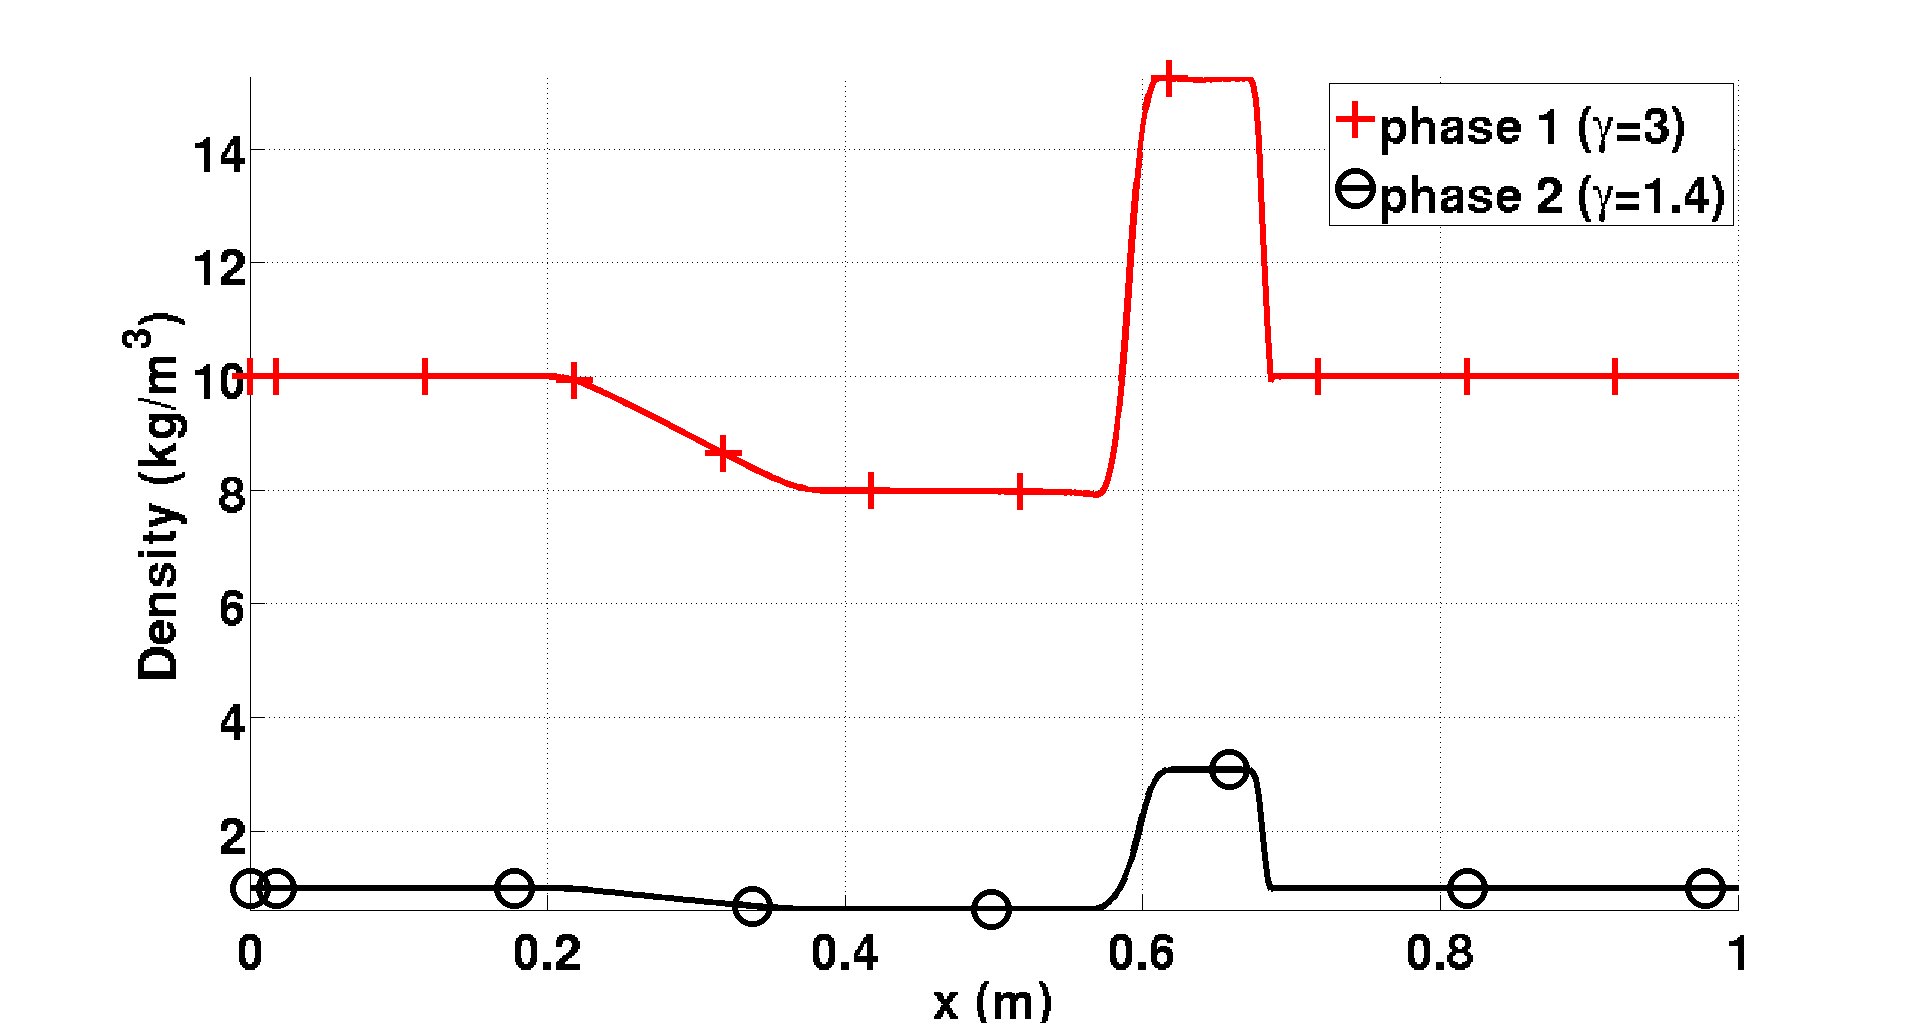
\includegraphics[width=\textwidth]{figures/relaxation_two_phases_density.png}
                \caption{Velocity}
                \label{fig:inf-rel-vel}
        \end{subfigure}%
        \begin{subfigure}[b]{0.495\textwidth}
                \centering
                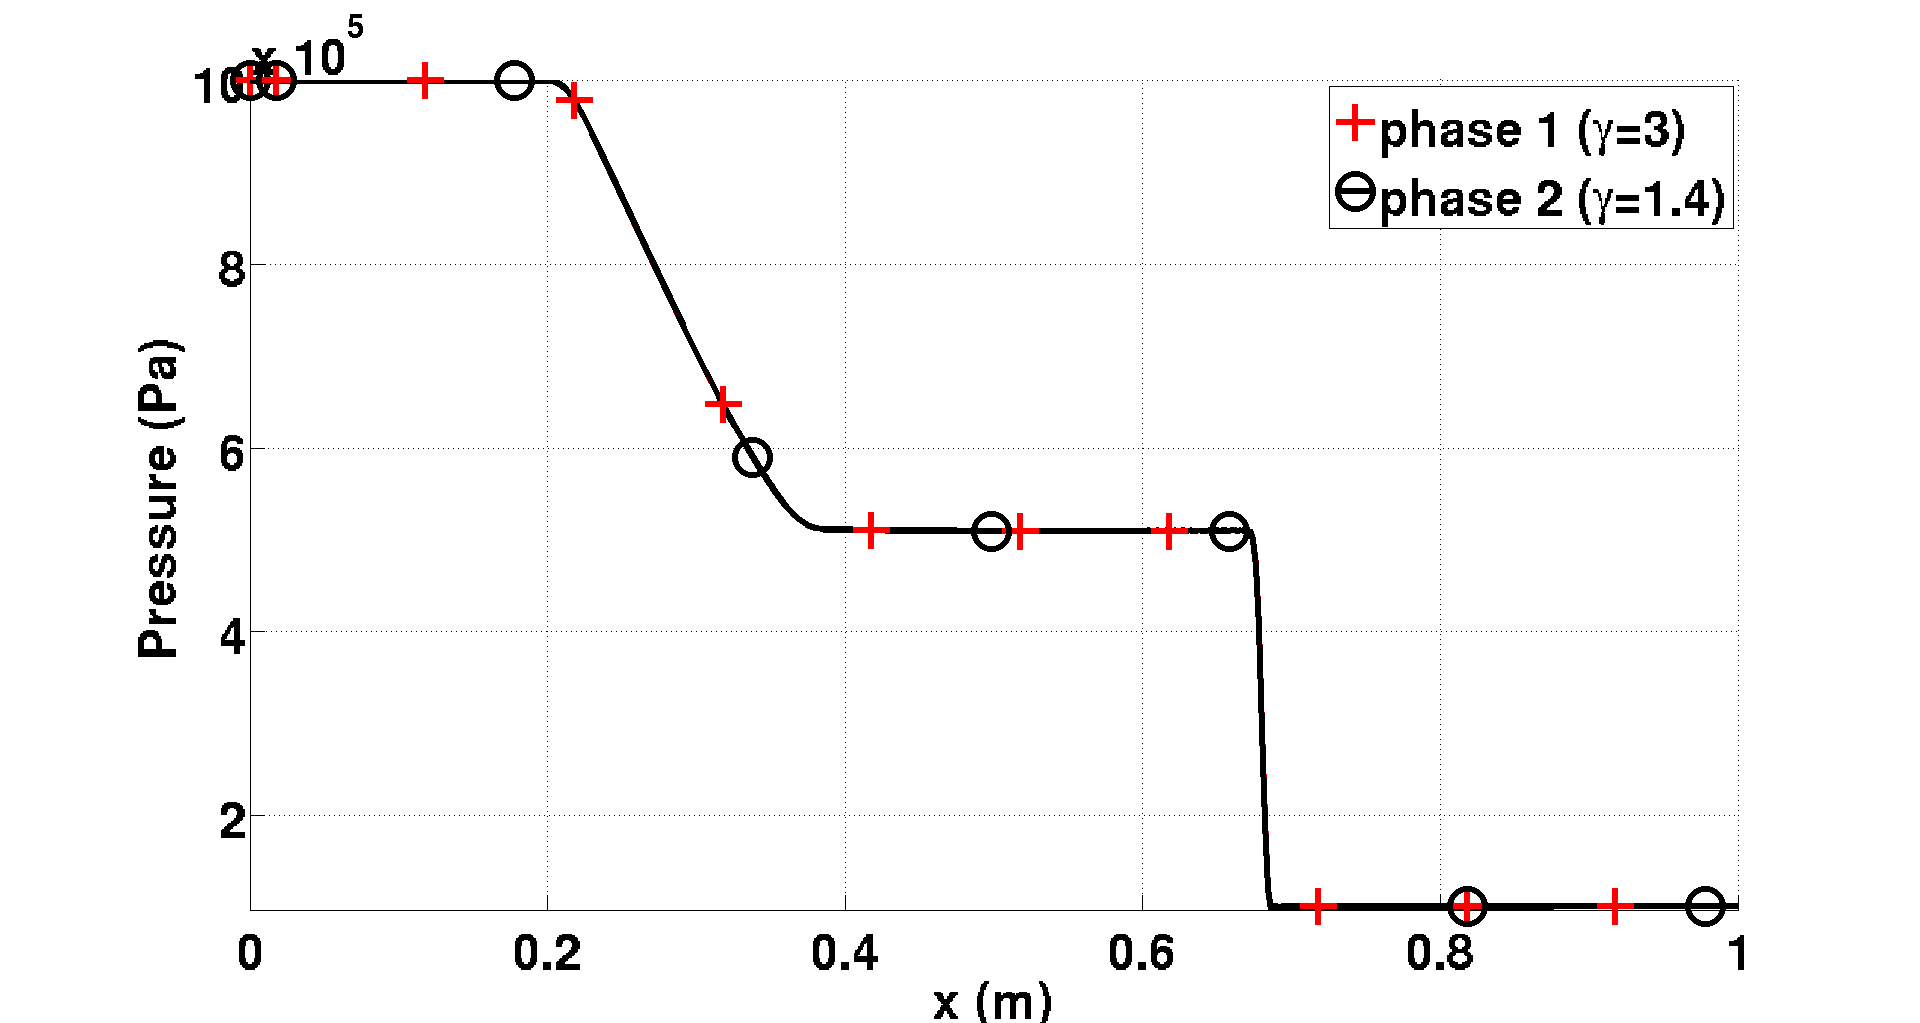
\includegraphics[width=\textwidth]{figures/relaxation_two_phases_pressure.png}
                \caption{Density}
                \label{fig:inf-rel-density}
        \end{subfigure}
        
        \begin{subfigure}[b]{0.495\textwidth}
                \centering
                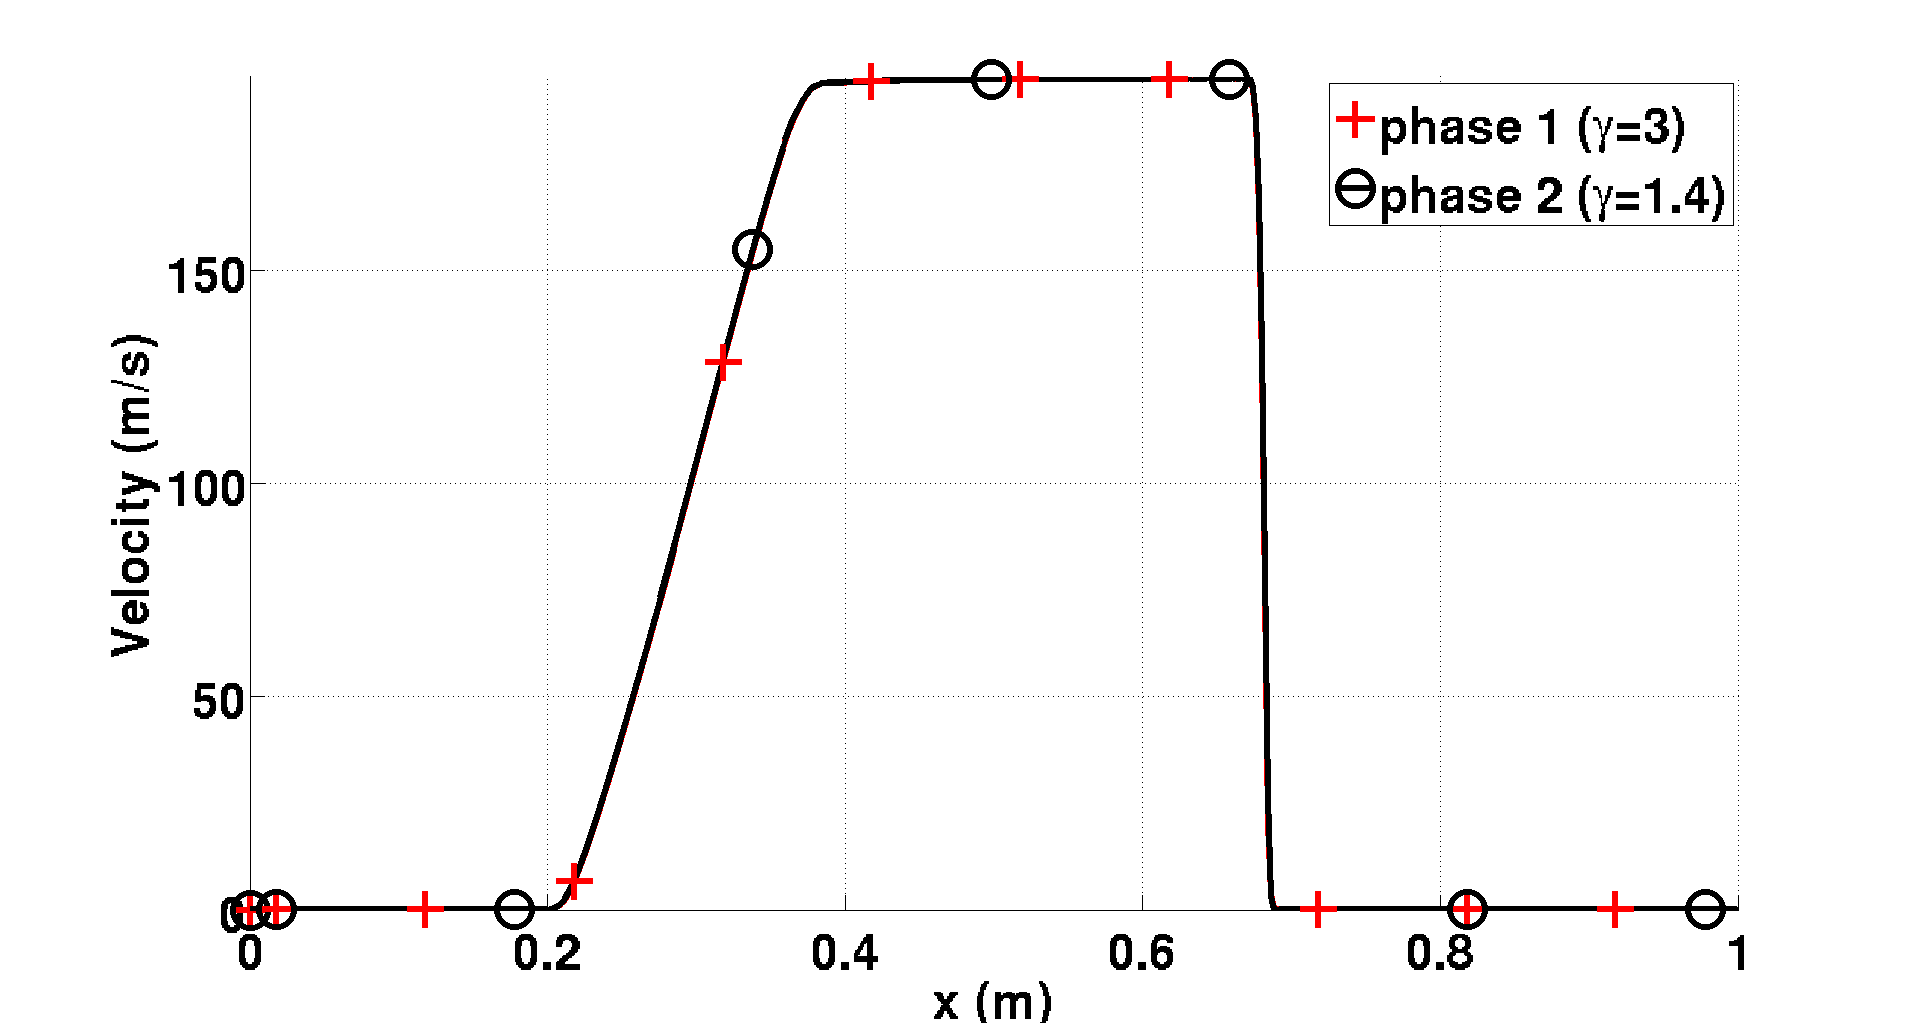
\includegraphics[width=\textwidth]{figures/relaxation_two_phases_velocity.png}
                \caption{Pressure}
                \label{fig:inf-rel-press}
        \end{subfigure}        
        \begin{subfigure}[b]{0.495\textwidth}
                \centering
                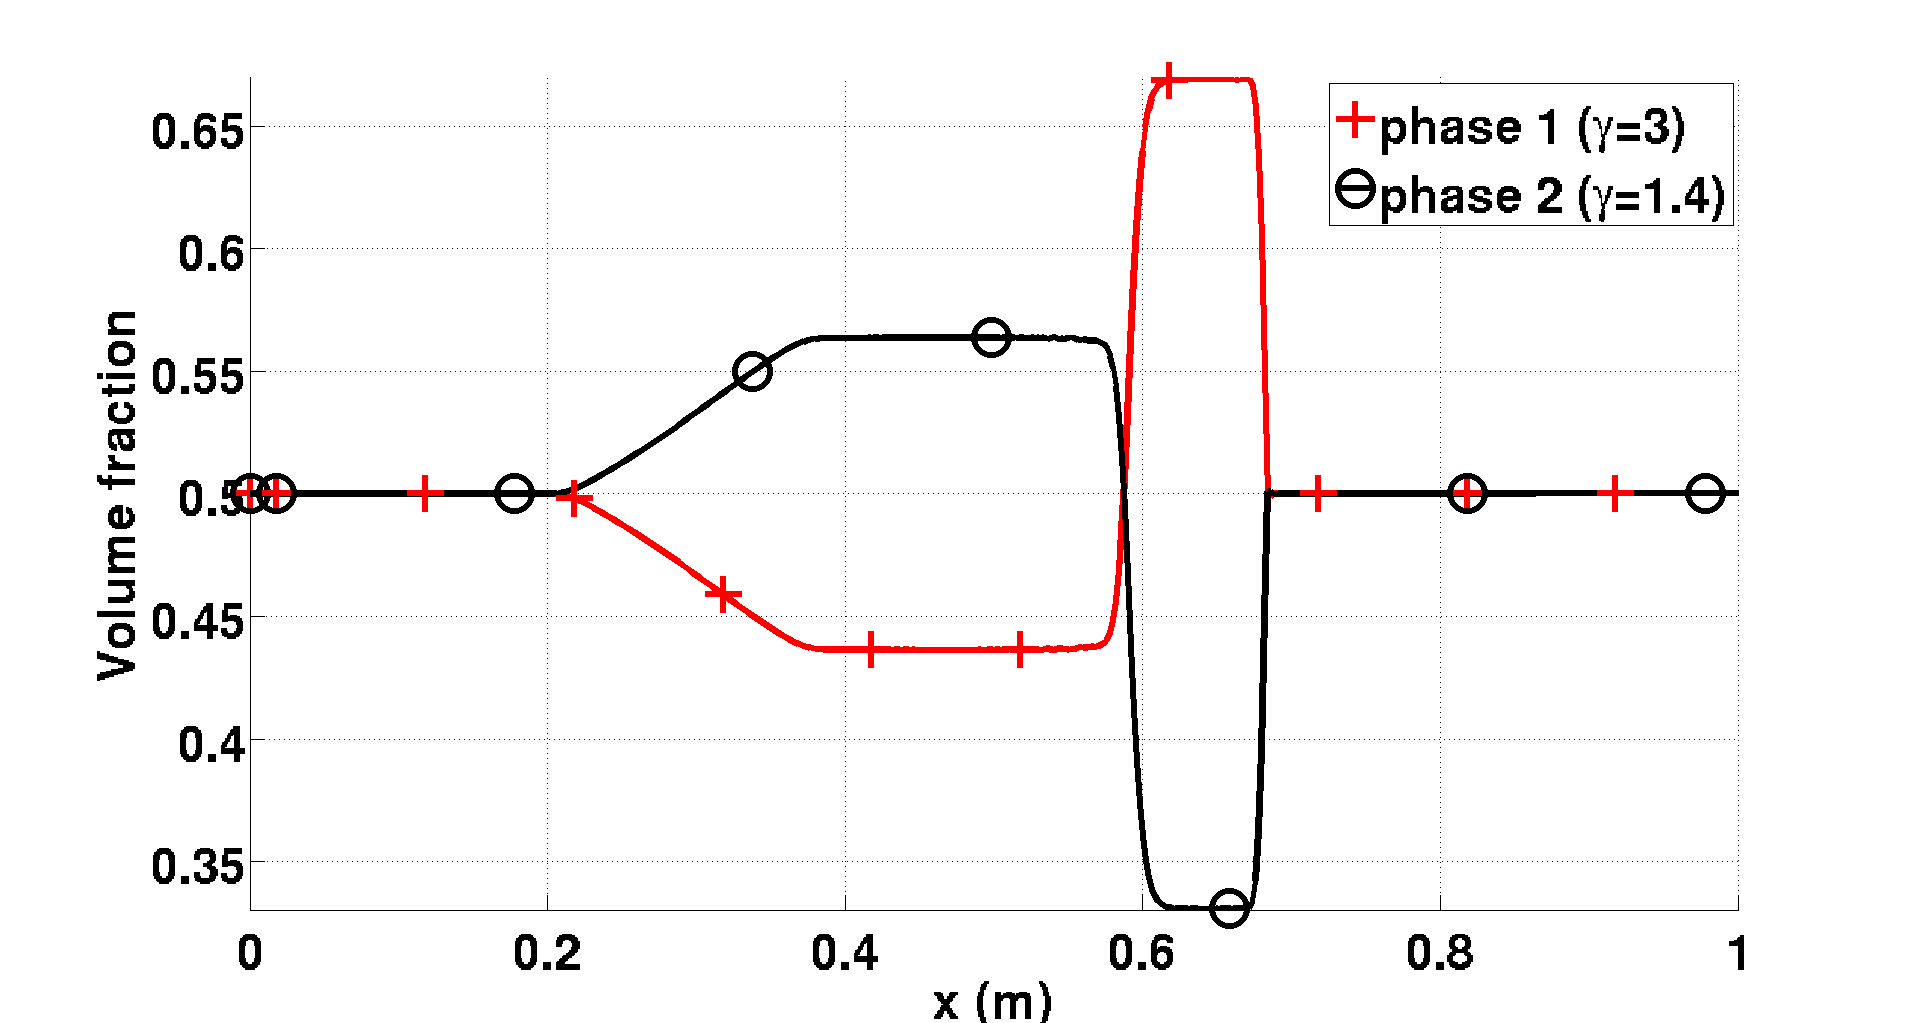
\includegraphics[width=\textwidth]{figures/relaxation_two_phases_volume_fraction.png}
                \caption{Volume fraction}
                \label{fig:inf-rel-vf}
        \end{subfigure}
        \caption{Numerical solution of a two-phase flow with large relaxation coefficients at $t=305 \ \mu s$.}\label{fig:inf-rel-variables}
\end{figure}
%
\begin{figure}[H]
        \centering
        \begin{subfigure}[b]{0.495\textwidth}
                \centering
                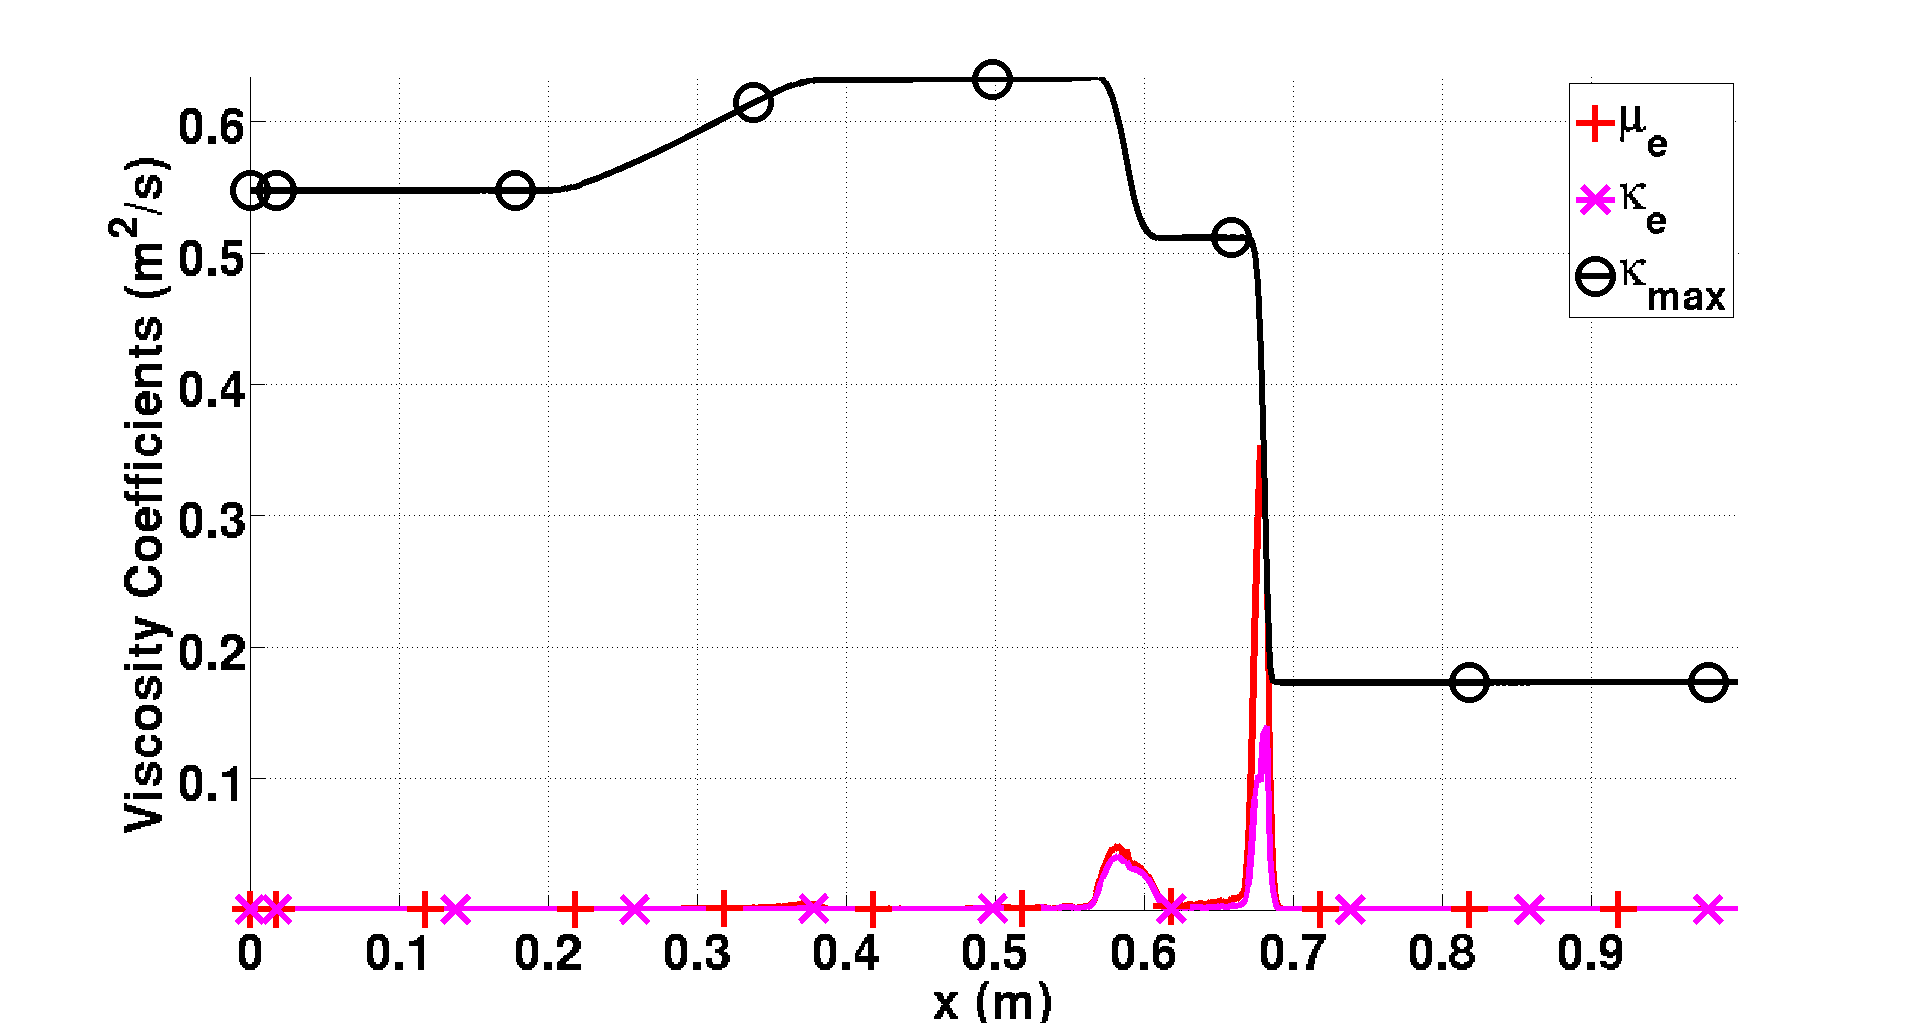
\includegraphics[width=\textwidth]{figures/relaxation_phase_1_viscosity_kappa_mu.png}
                \caption{Viscosity coefficients for phase 1.}
                \label{fig:inf-rel-visc-coeff-phase-1}
        \end{subfigure}%
        \begin{subfigure}[b]{0.495\textwidth}
                \centering
                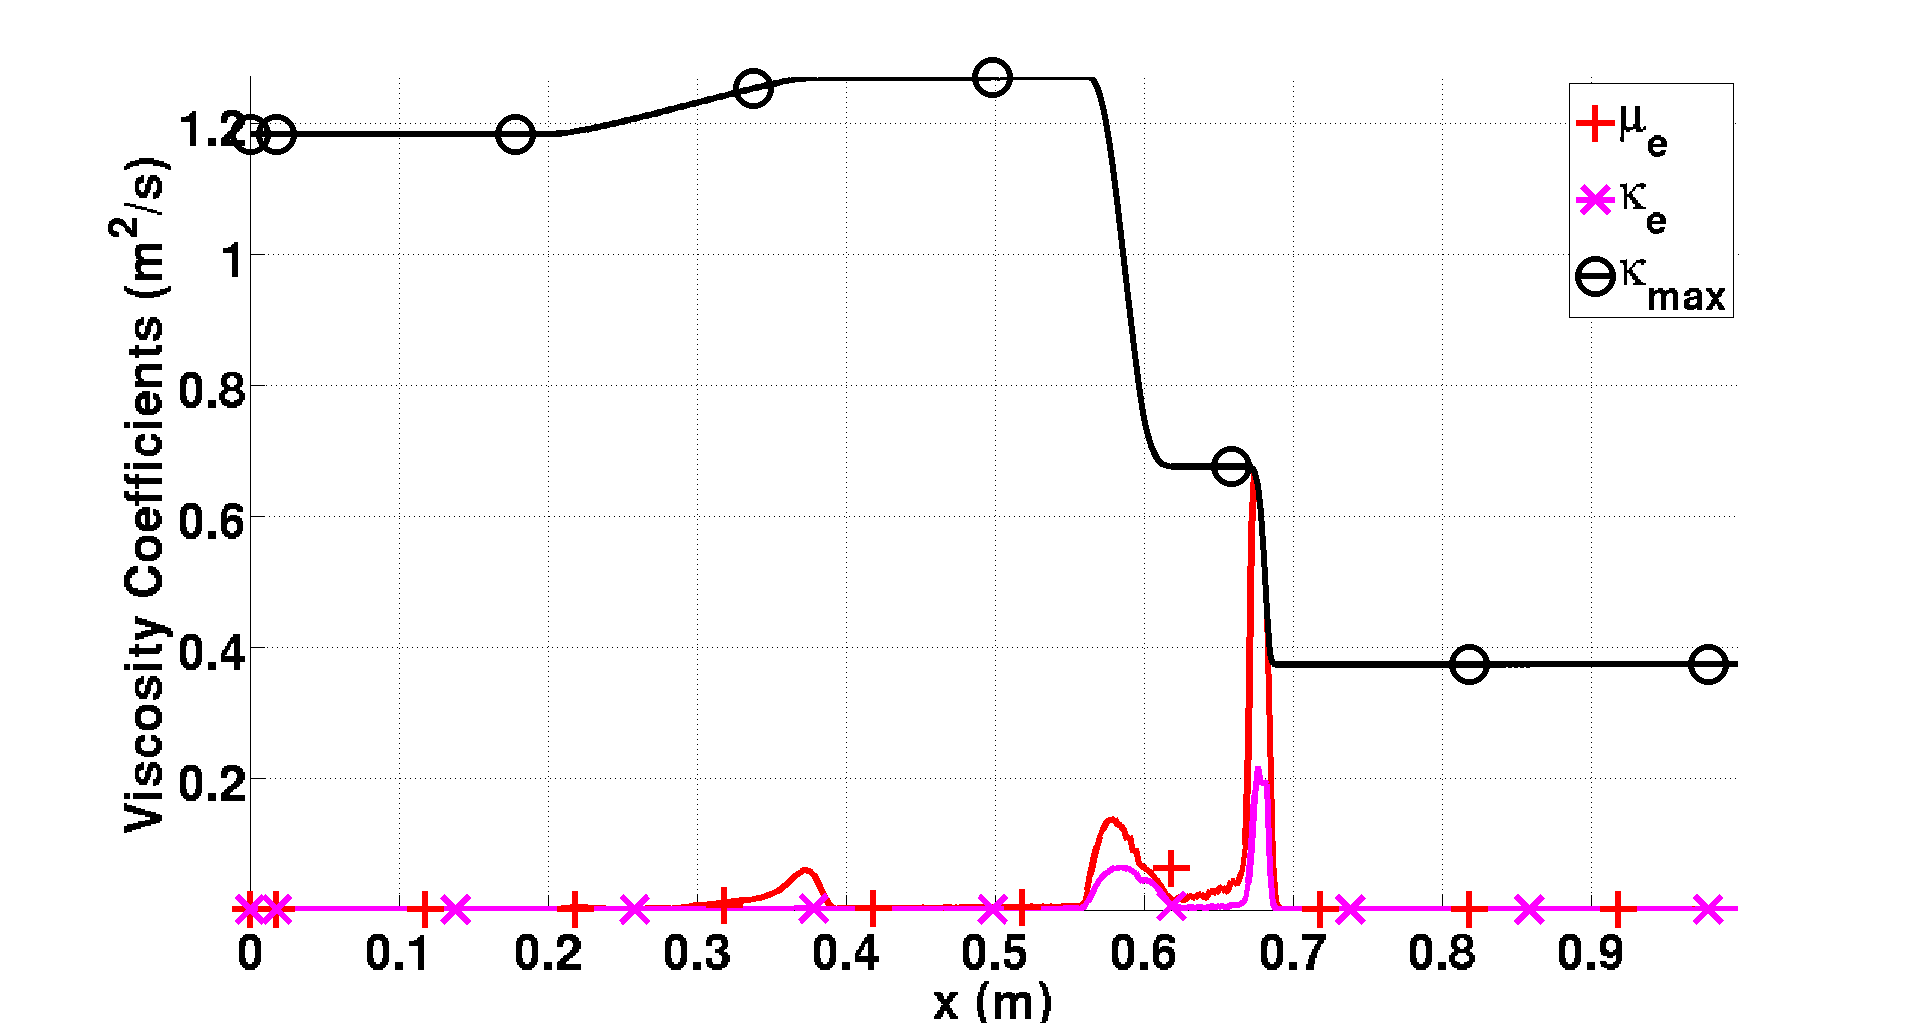
\includegraphics[width=\textwidth]{figures/relaxation_phase_2_viscosity_kappa_mu.png}
                \caption{Viscosity coefficients for phase 2}
                \label{fig:inf-rel-visc-coeff-phase-2}
        \end{subfigure}
        
        \begin{subfigure}[b]{0.495\textwidth}
                \centering
                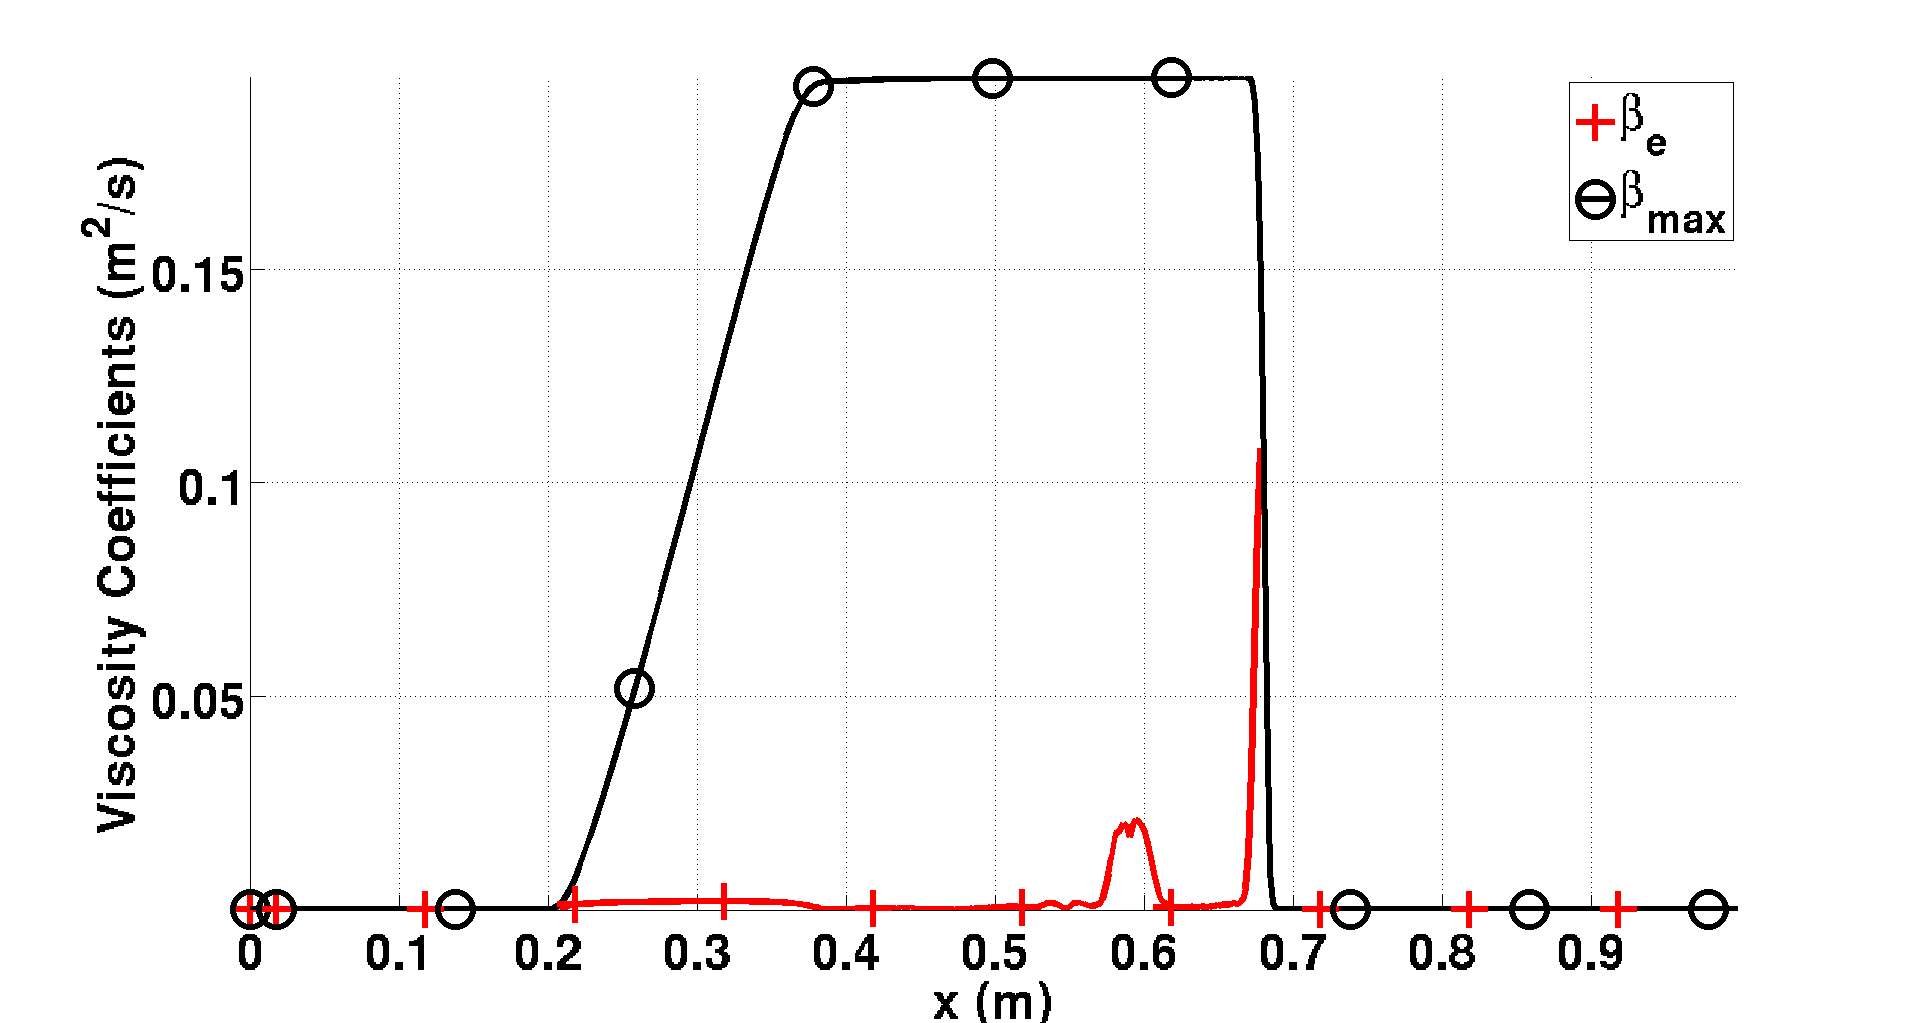
\includegraphics[width=\textwidth]{figures/relaxation_phase_1_beta.png}
                \caption{Viscosity coefficients for the volume fraction equation of phase 1.}
                \label{fig:inf-rel-beta}
        \end{subfigure}        
        \caption{Viscosity coefficients profiles for a two-phase flow with large relaxation coefficients at $t=305 \ \mu s$.}\label{fig:inf-rel-visc-coeff}
\end{figure}
%
%%%%%%%%%%%%%%%%%%%%%%%%%%%%%%%%%%%%%
\subsubsection{Two independent fluids in a 1-D converging-diverging nozzle}\label{sec:nozzle-two-indep-fluids}
%%%%%%%%%%%%%%%%%%%%%%%%%%%%%%%%%%%%%
%
In this test, we propose to investigate the behavior of two fluids in a one meter long 1-D converging-diverging nozzle with $A(x) = 1 + 0.5 \cos \left( 2\pi x \right)
$. This test was first introduced by Saurel et al. in \cite{SEM} for the 1-D seven-equation model and consists of a mixture of liquid water and vapor described 
by the SGEOS with the parameters given in \tbl{tbl:stff_gas_eos-sect4}.
%
\begin{table}[H]
\begin{center}
\caption{ Stiffened Gas Equation of State (SGEOS) parameters for steam and liquid water.}
\label{tbl:stff_gas_eos-sect4}
\begin{tabular}{|c|c|c|c|c|}
 \hline
\text{fluid}                           & $\gamma$ & $C_v$ $(J.kg^{-1}.K^{-1})$ & $P_\infty$ $(Pa)$ & $q$ $(J.kg^{-1})$ \\  \hline \hline
liquid water & 2.35     & 1816                       & $10^9$            & $-1167\ 10^3$     \\  \hline
steam          & 1.43     & 1040                       & 0                 & $ 2030\ 10^3$     \\  \hline
\end{tabular}
\end{center}
\end{table}
%
Stagnation boundary conditions are specified on the left of the nozzle (inlet) for both phases with a stagnation temperature $T_0 = 453 $ $K$ and a stagnation 
pressure $P_0 = 1$ $MPa$ (the stagnation density can be computed from $T_0$ and $P_0$ and the equation of state). At the outlet, a static pressure 
boundary condition is specified with $P = 0.5$ $MPa$ for both phases. The volume fraction is set to $\alpha_k = 0.5$ at the inlet. The initial conditions are 
computed from the boundary conditions by assuming the two fluids at rest and linearly interpolating the pressure and temperature between the boundary 
values. The geometry is discretized with an uniform mesh of 100 cells and run until steady state. The pressure and velocity relaxation coefficients are 
computed from EQUATION and EQUATION and the use of EQUATION for different values of $A_{int,max}$ that will be specified. 
%
%%%%%%%%%%%%%%%%%%%%%%%%%%%%%%%%%%%%%
\subsubsection{Fluids in a 1-D converging-diverging nozzle with infinite relaxation terms}\label{sec:nozzle-infinite-rel-coeff}
%%%%%%%%%%%%%%%%%%%%%%%%%%%%%%%%%%%%%
%
%
\subsection{1-D numerical results obtained with Relap-7}\label{sec:1d-results-relap-7}
%
%
\subsubsection{A two-phase flow water hammer test}\label{sec:water-hammer}
%
%
\subsubsection{A hydrostatic test}\label{sec:}
%
%
\subsection{Steady-state numerical solution of a Water Boiling Reactor (BWR)}\label{sec:bwr}
%
%%%%%%%%%%%%%%%%%%%%%%%%%%%%%%%%%%%%%%%%%%%%%%%%%%%%%%%%%%%%%%%%%%%%%%%%%%%%%
%%%%%%%%%%%%%%%%%%%%%%%%%%%%%%%%%%%%%%%%%%%%%%%%%%%%%%%%%%%%%%%%%%%%%%%%%%%%%
\section{Conclusions and future work}\label{sec:conclusion}
%%%%%%%%%%%%%%%%%%%%%%%%%%%%%%%%%%%%%%%%%%%%%%%%%%%%%%%%%%%%%%%%%%%%%%%%%%%%%
%%%%%%%%%%%%%%%%%%%%%%%%%%%%%%%%%%%%%%%%%%%%%%%%%%%%%%%%%%%%%%%%%%%%%%%%%%%%%
\bibliography{mybibfile}
\end{document}